\documentclass[12pt, oneside]{article}
\usepackage{amsmath,amssymb}
\usepackage[left=2.5cm, top=2.5cm, bottom=2.5cm, right=2.5cm]{geometry}

\usepackage{hyperref}
\hypersetup{
    colorlinks=true,
    linkcolor=blue,
    filecolor=magenta,      
    urlcolor=cyan,
}

\usepackage[utf8]{inputenc}
\usepackage[T1]{polski}
\usepackage[polish]{babel}
\usepackage{amsfonts}
\usepackage{subfig}
\usepackage[ruled]{algorithm2e}
\usepackage{graphicx}
\usepackage{wrapfig}
\graphicspath{ {images/} }

\usepackage{float}
\linespread{1.2}

\begin{document}  
\thispagestyle{empty}
\begin{titlepage}
    \begin{center}

           \Large
	\textbf{Uniwersytet Jagielloński w~Krakowie}\vspace{0.2cm}\\ Wydział Fizyki, Astronomii i~Informatyki Stosowanej
               \vspace*{1cm}
               
         \vspace{3cm}
         \Large
          \textbf{Piotr Kucharski}\\\vspace{0.5cm}
         \normalsize Nr albumu: 1124564\\
             \vspace{2cm}
        \Huge
        \textbf{Uczenie agentów sterowania pojazdami kosmicznymi}
      
        \vspace{1.5cm}
        \normalsize
        Praca licencjacka\\
        na kierunku Informatyka Stosowana\\ \vspace{0.15cm}
        
        \vfill
        \vspace{2cm}
       \begin{minipage}{1\textwidth}
\begin{flushright}
Praca wykonana pod kierunkiem\\
prof. dr. hab. Piotra Białasa\\
Zakład Technologii Gier
\end{flushright}
\end{minipage}
        
        \vspace{2cm}
        \begin{center}
      Kraków 2020
        \end{center}
    \end{center}
\end{titlepage}

\newpage 
 \thispagestyle{empty}
\vspace{2.5cm}
\begin{flushleft}
\large \textbf{Oświadczenie autora pracy}\vspace{0.6cm}\\
\end{flushleft}

\noindent Świadom odpowiedzialności prawnej oświadczam, że niniejsza praca dyplomowa została napisana przeze mnie samodzielnie i~nie zawiera treści uzyskanych w~sposób niezgodny z~obowiązującymi przepisami.\\

\noindent Oświadczam również, że przedstawiona praca nie była wcześniej przedmiotem procedur związanych z~uzyskaniem tytułu zawodowego w~wyższej uczelni.
\vspace{2cm}
\begin{center}
\begin{tabular}{lr}
................................~~~~~~~~~~~~~~~~~~~~~~~~~~~~~~~~~~~~~~&
.......................................... \\
{~~~~Kraków, dnia} & {Podpis autora pracy~~~~}
\end{tabular}
\end{center}
\vspace{5cm}
\begin{flushleft}
\large \textbf{Oświadczenie kierującego pracą}
\end{flushleft}

\noindent Potwierdzam, że niniejsza praca została przygotowana pod moim kierunkiem i~kwalifikuje się do przedstawienia jej w~postępowaniu o~nadanie tytułu zawodowego.
\vspace{2cm}
\begin{center}
\begin{tabular}{lr}
................................~~~~~~~~~~~~~~~~~~~~~~~~~~~~~~~~~~~~~~&
............................................ \\
{~~~~Kraków, dnia} & {Podpis kierującego pracą~~}
\end{tabular}
\end{center}
\vfill
\newpage
\tableofcontents
\newpage
\section{Abstrakt}
W~niniejszej pracy przedstawiam wynik serii eksperymentów mających na celu zbadanie skuteczności i~niezawodności prostego wariantu algorytmu uczenia ze wzmocnieniem Deep Q-Networks\cite{mnih2013playing}. Zadaniem algorytmu jest uczenie sztucznej sieci neuronowej sterowania pojazdami w~symulowanej przestrzeni kosmicznej. Z~przeprowadzonych eksperymentów wynika, że algorytm jest skuteczny w~znajdywaniu dobrych strategii w~prostych środowiskach podczas gdy w~bardziej skomplikowanych środowiskach algorytm rzadziej znajduje dobre strategie, a~parametry muszą być precyzyjnie dobierane.

\section{Wstęp}
Uczenie nadzorowane, najczęściej wykorzystywany rodzaj uczenia maszynowego, polega na uczeniu funkcji na podstawie zbioru danych wejściowych i oczekiwanego wyniku. Po predykcji wyniku na podstawie danych wejściowych poznawana jest dokładna wartość popełnionego błędu.  
Uczenie ze wzmocnieniem polega na uczeniu funkcji na podstawie interakcji ze środowiskiem. Dane wejściowe są obserwowane podczas symulacji, a~całkowita nagroda(błąd) poznawana jest dopiero po zakończeniu symulacji.
Przykładem może być np. nauka gry w~szachy, gdzie dopiero po zakończeniu gry poznajemy  wynik. Nie mamy jednak informacji o~wartości poszczególnych ruchów przez co jest to dużo bardziej skomplikowany problem. 
Algorytm Atari DQN\cite{mnih2013playing} był w~stanie nauczyć sztuczną sieć neuronową strategii podejmowania dobrych decyzji w~siedmiu grach na platformie Atari. Nauka kolejnych gier Atari nie wymagała modyfikacji w~algorytmie. Moim celem w~tej pracy jest zbadanie skuteczności algorytmu w~znajdywaniu dobrych strategii w~trzech środowiskach.

\section{Środowisko}
Agent podlegający uczeniu steruje pojazdami poruszającymi się po dwuwymiarowej, ciągłej przestrzeni kosmicznej. 
Pojazdy poruszają się zgodnie z~zasadami dynamiki Newtona, bez oporów wpływających na ich aktualną prędkość. 
Środowisko, napisane w~C++, jest kontrolowane przez agenta, napisanego w~Pythonie. 
Interfejs komunikacji środowiska z~agentem składa się trzech funkcji: funkcji aktualizacji stanu środowiska, funkcja pozwalająca przywrócić środowisko do stanu początkowego oraz funkcji zwracającej informację o~tym, czy środowisko jest nadal aktywne. Funkcja aktualizacji środowiska przyjmuje na wejściu akcje i~zwraca następny stan, nagrodę oraz informacje o~tym, czy pojazd został zresetowany. Funkcja resetująca środowisko do stanu początkowego zwraca tylko stan.

\subsection{Akcje}
Przy każdej aktualizacji środowiska zadaniem agenta jest kontrolowanie ruchu pojazdu poprzez wybranie jednej z~możliwych akcji. Wybrana przez agenta akcja odpowiada z~jaką mocą mają działać dwa silniki. Pierwszy silnik nadaje przyspieszenie w~kierunku przodu pojazdu, drugi przyspieszenie obrotowe. 
Pierwszy silnik posiada dwie możliwe akcje: wyłączony albo włączony $[0,1]$. 
Drugi silnik posiada trzy możliwe akcje: lewo, wyłączony, prawo $[-1,0,1]$. 
Przestrzeni akcji powstaje z~iloczynu kartezjańskiego zbiorów możliwych akcji obu silników. Z~przestrzeni akcji usuwana jest akcja neutralna, kiedy oba silniki są wyłączone, gdyż w~początkowym etapie uczenia ta akcja była faworyzowana, co prowadziło do stagnacji procesu uczenia. 

\subsection{Stan}
Agent podejmuje decyzję którą akcję wykonać w~danym kroku na podstawie stanu otrzymanego ze środowiska. 
Stan obserwowany przez agenta w~składa się z~trzech liczb rzeczywistych odpowiadających kolejno szybkości pojazdu, kątowi pomiędzy kierunkiem statku a~wektorem prędkości oraz prędkości kątowej.
\begin{equation}
\begin{aligned}
&1)~|Velocity|\\
&2)~\measuredangle{ShipDirection} - \measuredangle{Velocity}\\
&3)~AngularVelocity\\
\end{aligned}
\end{equation}
W~scenariuszach, w~których celem jest dotarcie pojazdem do wyznaczonego punktu kontrolnego, stan zawiera dodatkowo dwie liczby rzeczywiste odpowiadające odległości pojazdu od punktu kontrolnego oraz kątowi pomiędzy kierunkiem statku a~wektorem odległości do tego punktu.
\begin{equation}
\begin{aligned}
&4)~|CheckpointPosition - ShipPosition|\\
&5)~\measuredangle{ShipDirection} - \measuredangle{(CheckpointPosition - ShipPosition)}\\
\end{aligned}
\end{equation}

\subsection{Graficzna reprezentacja środowiska}
\begin{wrapfigure}[8]{l}{0.25 \textwidth}
\centering
\vspace{-25pt}
\caption{Pojazd.}
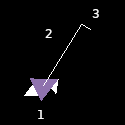
\includegraphics[width=0.25 \textwidth , height=0.25 \textwidth]{shipsingle2}
\label{poj}
\end{wrapfigure}
Na rysunku po lewej stronie pojazd 1 jest reprezentowany przez trzy trójkąty. Kolorowy trójkąt reprezentuje kadłub pojazd, a~jego najostrzejszy wierzchołek wskazuje przód. Dwa białe trójkąty pokazują włączone silniki. 
Trójkąt połączony z~krótszą krawędzią pojazdu reprezentuje główny silnik, a~trójkąt połączony z~przodem pojazdu reprezentuje silnik rotujący. 
Odcinki 2 - prędkości oraz 3 - prędkość obrotowa są graficzną reprezentacją stanu.
Do renderowania środowiska używam biblioteki SFML\cite{sfml}.

\subsection{Funkcja aktualizacji środowiska}
Po wybraniu przez agenta akcji następuje aktualizacja stanu środowiska.
Podczas kroku aktualizacji środowiska w~pierwszej kolejności obliczane jest przyspieszenie działające na pojazd, które zależy od wybranej przez agenta akcji decydującej o~mocy głównego silnika. 
Parametry pojazdu $mainEnginePower$, $mass$, $rotationEnginePower$ oraz $size$ są stałe.
\begin{equation}
\begin{aligned}
&\begin{cases}
Acceleration_x = firstAction * cos(ShipDirection) * mainEnginePower / mass \\
Acceleration_y = firstAction* sin(ShipDirection) * mainEnginePower / mass \\
\end{cases}\\
&~~Velocity = Velocity + Acceleration * timeStep \\
&~~ShipPosition = ShipPosition + Velocity * timeStep\\
\end{aligned}
\end{equation}
Po zaktualizowaniu położenia pojazdu obliczana jest rotacja pojazdu.
\begin{equation}
\begin{aligned}
&AngularAcceleration = secondAction * rotationEnginePower / (0.5*mass*size)\\
&AngualarVelocity = AngualarVelocity + AngularAcceleration * timeStep\\
&ShipDirection = ShipDirection + AngularVelocity * timeStep
\end{aligned}
\end{equation}
Środowisko aktualizowane jest ze stałym krokiem czasowym wynoszącym dziesiątą część sekundy.
Po zaktualizowaniu położenia oraz rotacji pojazdu obliczana jest nagroda oraz sprawdzane są warunki kończące symulację pojazdu. 
Funkcja zwraca krotkę z~adresami pamięci, pod którymi znajdują się wektory zawierające następny stan, nagrodę oraz informację czy pojazd zakończył symulację w~tym kroku. Zmienne $firstAction$ oraz $secondAction$ przyjmują wartości 0 albo 1.
Do komunikacji pomiędzy Pythonem a~C++ z~biblioteki BOOST\cite{boost}. 

\subsection{Scenariusze i~modelowanie funkcji nagrody}
Na potrzeby eksperymentów zaimplementowałem trzy scenariusze różniące się pomiędzy sobą sposobem obliczania nagrody oraz poziomem trudności. 
\newline\newline
Celem pierwszego, najprostszego scenariusza jest nauczenie agenta zmniejszania szybkości rozpędzonego pojazdu. 
Pojazd rozpoczyna symulację posiadając losową rotację, losową prędkość obrotową z~zakresu $[-2,2]~rad/s$ oraz wektor prędkości, którego elementy losowane są z~zakresu $[5,10]~m/s$. 
Po każdej aktualizacji środowiska agent otrzymuje nagrodę odpowiadającą odwrotnej zmianie szybkości w~danym kroku $r_t=|Velocity_{t-1}|-|Velocity_t|$. 
Pojazd ulega zniszczeniu i~jest resetowany gdy jego szybkość przekroczy $20~m/s$ lub gry szybkość obrotowa przekroczy $2~rad/s$. Agent otrzymuje karę za wybranie akcji prowadzącej do zniszczenia pojazdu.
Gdy szybkość pojazdu zmaleje poniżej $2~m/s$ agent otrzymuje nagrodę za zaliczenie scenariusza i ocalenie pojazdu. Otrzymywana przez agenta nagroda/kara po osiągnięciu stanu terminalnego we wszystkich scenariuszach wynosi $\pm1$.
\newline\newline
Celem drugiego i~trzeciego scenariusza jest nauczenie agenta dolatywania pojazdem do wyznaczonego losowo punktu kontrolnego. Podobnie jak w~pierwszym scenariuszu pojazd na początku posiada losową rotację, prędkość obrotową $[-1,1]~rad/s$, oraz elementy wektora prędkości losowane z~zakresu $[0,10]~m/s$.  Startową pozycją pojazdu jest środek układu współrzędnych. Współrzędne punktu kontrolnego losowane są z~zakresu $[-700,700]~m$.
Gdy pojazd zbliży się do punktu kontrolnego na odległość mniejszą niż $25~m$ agent otrzymuje nagrodę, a~pojazd oraz punkt kontrolny są losowane na nowo, .
Gdy pojazd oddali się od punktu kontrolnego na więcej niż $1400~m$ lub jego szybkość obrotowa przekroczy $2~rad/s$ agent otrzymuje karę, pojazd ulega zniszczeniu a~punkt kontrolny pozostaje w~tym samym miejscu. 
W~drugim scenariuszu nagroda otrzymywana przez agenta po każdej aktualizacji odpowiada odwrotnej zmianie odległości pojazdu od punktu kontrolnego $r_t = d_{t-1}-d_t$, gdzie $d_t$ odpowiada odległości euklidesowej pojazdu od punktu kontrolnego w~kroku $t$. 
W~trzecim scenariuszu nagroda odpowiada zmianie szybkości w~kierunku punktu kontrolnego $r_t = d_{t-2} - 2*d_{t-1} + d_t$.

\section{Definicja uczenia ze wzmocnieniem}
Uczenie ze wzmocnieniem polega na optymalizacji strategii wybierania akcji na podstawie doświadczeń generowanych podczas interakcji ze środowiskiem. Matematycznym sformułowaniem procesu interakcji agenta ze środowiskiem jest proces decyzyjny Markowa. Proces ten składa się z~krotki $(S, A, P, R)$, gdzie $S$ to zbiór stanów środowiska w~jakich może się znaleźć symulowany pojazd, $A$ to zbiór akcji, $P(s'|s,a)$ to rozkład prawdopodobieństwa przejścia pomiędzy stanami w~zależności od wybranej akcji, $R(s,a)$ to funkcja nagrody otrzymywanej przez agenta natychmiast po wykonaniu akcji w~zadanym stanie.
Proces interakcji ze środowiskiem tworzy serię doświadczeń $s_1, a_1, r_1, s_2, a_2, r_2 ... s_T, a_T, r_T$, gdzie $T$ oznacza numer kroku terminalnego, w~którym kończy się epizod i~symulacja pojazdu jest resetowana.
Obniżona nagroda geometrycznie zmniejsza wartość nagród otrzymywanych w~następnych krokach. 
\begin{equation}
R_t=\sum^T_{i=t} \gamma^{(i-t)}r_i
\end{equation}
Parametr zniżki $0<\gamma<1$ zmniejszając przyszłe nagrody przeciwdziała zbieganiu sumy nagród do nieskończoności oraz wymusza na agencie wybieranie dobrych akcji wcześniej zamiast je odwlekać.
%\begin{equation}
%P(s'|s,a) = \mathbb{P}[S_{t+1}=s'|S_t=s,A_t=a]
%\end{equation}
Maksymalna obniżona nagroda możliwa do uzyskania z~danego stanu zdefiniowana jest jako optymalna funkcja wartości.
\begin{equation}
V^*(s)=\max_a[R(s,a)+ \gamma \sum_{s'}P(s'|s,a)V^*(s')]
\end{equation}
Maksymalna oczekiwana nagroda do uzyskania z~danego stanu po podjęciu określonej akcji to optymalna funkcja wartości akcji $Q^*$. 
\begin{equation}
Q^*(s,a)=R(s,a)+ \gamma \sum_{s'}P(s'|s,a) \max_{a'} Q^*(s',a')
\end{equation}
\begin{equation*}
V^*(s)= \max_a Q^*(s,a)
\end{equation*}
Strategię $\pi$ zdefiniowana jest jako funkcja rozkładu prawdopodobieństwa akcji na zadanym stanie. 
\begin{equation}
\pi(a|s)=\mathbb{P}[a_t=a|s_t=s]
\end{equation} 
Jeśli, tak jak w~przypadku tej pracy, strategia jest deterministyczna, to zwraca ona wartość $1$ dla wybranej akcji i~$0$ dla wszystkich pozostałych.
Optymalna strategia $\pi^*$ w~każdym stanie $s \in S$ wybierze taką akcję $a$, która maksymalizuje obniżoną nagrodę. Jeśli optymalna wartość $Q^*(s',a')$ w~następnym kroku jest znana dla wszystkich możliwych akcji $a'$, to optymalną strategią podejmowania akcji jest wybieranie $a'$ maksymalizując oczekiwaną obniżoną nagrodę. 
\begin{equation}
\pi^*(s)=arg\max_aQ^*(s,a)
\end{equation} 
Funkcję wartości oraz funkcję wartości akcji można zdefiniować dla dowolnej polityki $\pi$.
\begin{equation}
V_\pi(s)= \sum_a \pi(a|s)[R(s,a)+ \gamma \sum_{s'}P(s'|s,a)V_\pi(s')]
\end{equation}
\begin{equation}
Q_\pi(s,a) =R(s,a) + \gamma \sum_{s'}P(s'|s,a)\sum_{a'}\pi(a'|s')Q_\pi(s',a')
\end{equation}
%\begin{equation*}
%V_\pi(s)=\sum_{a}\pi(a|s)Q_\pi(s,a)
%\end{equation*}
%Podczas uczenia dążymy do minimalizacji funkcji kosztu Temporal Difference\cite{sutton}.
%\begin{equation}
%TD=R_t - Q(s,a)
%\label{td}
%\end{equation}
Podczas uczenie dążymy do strategii dającej najwyższą możliwą obniżoną nagrodę.
\begin{equation}
Q^*(s,a)=\max_\pi Q_\pi (s,a)
\label{td}
\end{equation}
Równanie (\ref{td}) można rozwiązać iterując poniższe równanie (\ref{qoptim}). Parametr $\alpha$ opisuje wielkość kroku optymalizacyjnego. Taka iteracja funkcji wartości akcji zbiega do optymalnej funkcji $Q_i \rightarrow Q^* $ dla $ i~\rightarrow \infty$\cite{sutton}.
\begin{equation}
Q_{i+1}(s,a)=Q_t(s,a)+\alpha[R(s,a)+\gamma \sum_{s'}P(s'|s,a) \max_{a'} Q_t(s',a') - Q_t(s,a)]
\label{qoptim}
\end{equation}
%\begin{equation}
%Q_{i+1}(s,a)=Q_t(s,a)+\alpha[R(s,a)+\gamma \sum_{s'}P(s'|s,a) \max_{a'} Q_t(s',a') - Q_t(s,a)]
%\label{td}
%\end{equation}
W~przypadku tej pracy takie podejście jest niewykonalne, gdyż przestrzeń stanów jest za duża, agent nie zna funkcji $P(s'|s,a)$, epizody mogą być bardzo długie oraz chcemy, żeby funkcja $Q$ była uczona w~trakcie trwania symulacji, a~nie dopiero po jej zakończeniu.

\section{Głębokie uczenie funkcji wartości akcji $Q$}
Bez dostępu do funkcji przejścia $P(s'|s,a)$ proces optymalizacji bazuje na seriach doświadczeń generowanych podczas interakcji ze środowiskiem. Wszystkie doświadczenia, razem z~następnym zaobserwowanym stanem $s'$, są zapisywane w~pamięci $M$. Funkcja wartości jak i~funkcja wartości akcji opiera się na założeniu, że kolejne akcje w~serii były wybierane zgodnie ze strategią $\pi$. 
\begin{equation}
V_\pi(s)= \mathbb{E}[r_t+ \gamma V_\pi(s_{t+1})|s_t=s, a_t \sim \pi(s_t)]
\end{equation}
\begin{equation}
Q_\pi(s,a) = \mathbb{E}[r_t + \gamma Q_\pi(s_{t+1},a_{t+1})|s_t=s,a_t=a, \pi]
\end{equation}
Celem znalezienia optymalnej strategii korzystam ze sztucznej sieci neuronowej z~parametrami $\theta$, której zadaniem jest uczenie optymalnej funkcji wartości akcji $Q(s,a: \theta ) \approx Q^*(s,a)$. Sieć neuronową można uczyć minimalizując sekwencje funkcji kosztu $L_i(\theta_i)$. Funkcja kosztu odpowiada kwadratowi błędu z funkcji (\ref{qoptim}) $R(s,a)+\gamma \sum_{s'}P(s'|s,a) \max_{a'} Q_t(s',a') - Q_t(s,a)$ z~tą różnicą, że stan $s$, akcja $a$, nagroda $r$ oraz następny stan otrzymany po aktualizacji środowiska $s'$ są losowane z~pamięci doświadczeń $M$.
\begin{equation}
L_i(\theta_i) = \mathbb{E}_{s,a,r,s' \sim M}[(r+\gamma \max_{a'} Q(s',a':\theta_{i-1}) - Q(s,a:\theta_i))^2]
\end{equation}
Wagi sieci neuronowej optymalizuje się za pomocą stochastycznego spadku wzdłuż gradientu.
\begin{equation}
\nabla_{\theta_i}L_i(\theta_i)= \mathbb{E}_{s,a,r,s' \sim M}[(r+\gamma \max_{a'} Q(s',a':\theta_{i-1}) - Q(s,a:\theta_i))\nabla_{\theta_i}Q(s,a:\theta_i)]
\end{equation}
Wagi $\theta_{t-1}$ są podczas treningu zamrożone. Korzystanie z~wag z~poprzedniej aktualizacji mogłoby spowodować wybieranie tych samych nieoptymalnych akcji na podstawie poprzednich wag. Prowadzi to do katastroficznego zapominania. Z~tego powodu wagi $\theta_{t-1}$ są zastąpione wagami $\theta_f$, które co stałą liczbę kroków $target\_update\_frequency$ przyjmują wartość $\theta_t$.

\subsection{Problemy głębokiego uczenia ze wzmocnieniem}
Kolejne stany środowiska są bardzo do siebie podobne, co w~procesie uczenia prowadziłoby do zbiegania do nieoptymalnego lokalnego minimum. Celem uniknięcia tej sytuacji pamięć $M$ ma pojemność $memory\_size > 5 000$, a~partie do uczenia o~wielkości $b<<memory\_size$ są wybierane z~pamięci z~jednakowym prawdopodobieństwem $(S_b,A_b,R_b,S'_b) \sim M$. Prowadzi to do zwiększenia niezależności stanów, na podstawie których obliczany jest krok uczący. Drugim sposobem na zwiększenie niezależności i~różnorodności stanów jest jednoczesna nauka na podstawie wielu niezależnych pojazdów. Pojazdy inicjalizowane w~sposób losowy prowadzą do lepszej eksploracji przestrzeni stanów. Wyniki przeprowadzonych eksperymentów wskazują na znaczącą poprawę wyników uczenia już przy pięciu symulowanych jednocześnie pojazdach. Eksperymenty przeprowadziłem symulując jednocześnie 100 pojazdów.
\newline\newline
Gdyby agent od początku chciwie podejmował akcje na podstawie losowo zainicjalizowanej funkcji wartości akcji  $a_t=\max_aQ(s_t,a:\theta)$ mógłby, przez niedostateczną eksplorację, pozostać w~lokalnym minimum. Eksplorację wymusza się na agencie poprzez wybieranie z~prawdopodobieństwem $\epsilon$ losowej akcji $a_t \sim A$, a~z prawdopodobieństwem $1-\epsilon$ akcji chciwej $a_t=\max_aQ(s_t,a:\theta)$. Ten sposób podejmowania akcji nazywa się $\epsilon$-greedy\cite{sutton}. Wartość $\epsilon$ jest warunkowana początkową wartością $\epsilon_{start}$, końcową wartością $\epsilon_{end}$ oraz liczbą kroków  $\epsilon_{decay}$ po których $\epsilon$ ma osiągnąć wartość końcową. W~trakcie treningu $\epsilon$ zmniejsza się z~każdym krokiem zgodnie z~równaniem $\epsilon_t=\epsilon_{end} + (\epsilon_{start} - \epsilon_{end}) e^{(-t/\epsilon_{decay})}$. 
\newline \newline
Następnym problemem w~głębokim uczeniu ze wzmocnieniem są eksplodujące gradienty. Główną przyczyną eksplozji jest duże odchylenie standardowe obserwowanych nagród. Żeby przeciwdziałać eksplodującym gradientom korzystam z~funkcji kosztu $smooth\_ L1\_ loss$\cite{frnn}, która zmniejsza wpływ skrajnych pomiarów na całkowity gradient kroku uczącego.
\begin{equation}
smooth_{L_1}(x)=
\begin{cases}
0.5x^2 \qquad dla |x|<1\\
|x|-0.5 \quad dla |x| \geq 1
\end{cases}
\end{equation}
Podobnie jak w~Atari DQN\cite{mnih2013playing} korzystam z~optymalizatora $RMSprop$ zaproponowanego przez G. Hintona\cite{rmssource} a~po raz pierwszy opublikowanego w~pracy na temat optymalizacji rekurencyjnych sieci neuronowych służących do generowania tekstu\cite{rms}. 
%Optymizator przechowuje średnią kroczącą kwadratów gradientów dla każdej wagi $w \in \theta$, a~podczas aktualizacji wagi dzieli gradient przez pierwiastek kwadratowy tej średniej. 
\begin{equation}
\mathbb{E}[g^2]_t=\beta \mathbb{E}[g^2]_{t-1}+(1-\beta)(\frac{\delta L(x) }{ \delta w})^2
\end{equation}
\begin{equation}
w_t = w_{t-1}-\frac{\alpha}{\sqrt{\mathbb{E}[g^2]_t}} \frac{\delta L(x) }{ \delta w}
\end{equation}

\subsection{Sztuczna sieć neuronowa}
Funkcja aproksymująca $Q^*$  jest złożona z~wielu warstw funkjci liniowych zawierających nieliniowe aktywacje pomiędzy kolejnymi warstwami. Pierwsza funkcja liniowa przyjmuje na wejściu stan otrzymany ze środowiska, przekształca go na wektor o~wymiarze $width$ a~następnie oblicza nieliniową funkcję aktywacji $ReLu$\cite{relu} na wektorze wyjściowym. Kolejne $depth$ funkcji liniowych o~tej samej szerokości $width$ przekształca wektor w~ten sam sposób co pierwsza funkcja. Ostatnia funkcja liniowa przekształca wektor o~wymiarze $width$ na wektor wyjściowy  o~wymiarze odpowiadającym wielkości przestrzeni akcji $|A|$. Wartości wektora wyjściowego reprezentują wynik funkcji $Q_\pi(*|s)$. Korzystam z~algorytmów uczenia maszynowego zaimplementowanych w~bibiliotece PyTorch\cite{torch}.
\newpage
\subsection{Algorytm}
\begin{algorithm} 

 Inicjalizacja parametrów $\theta$ funkcji wartości akcji $Q$, $\theta_f = \theta$

 Inizjalizacja środowiska oraz otrzymanie pierwszego stanu$s_1$
 
 
 \For{t=0; t<T; t++}{
  Z~prawdopodobieństwem $\epsilon$ wybierz losową akcję $a_t \sim A $, 
  
  w~innym przypadku wybierz $a_t=\max_aQ(s_t,a:\theta)$
  
  Zaktualizuj stan środowiska wykonując akcję $a_t$ i~otrzymując $(r_t, s_{t+1})$
  
  Zapisz w~pamięci element $(s_t,a_t,r_t,s_{t+1})$
  
 
  \If{t>b}{
  	$(S_b,A_b,R_b,S'_b) \sim M$
  
  	Zaktualizuj wagi $\theta$ zgodnie z~$(R_b + \gamma \max_{a'} Q(S'_b,a':\theta_f)-Q(S_b,A_b:\theta))^2$
  }
   \If{(t \% częstotliwość aktualizacji $\theta_f$) == 0 }{
 $\theta_f = \theta$
 }
 }
 \caption{Głębokie uczenie Q-network z~wykorzystaniem pamięci}
\end{algorithm}

\section{System do przeprowadzania eksperymentów}
Chcąc przetestować w~jaki sposób algorytm uczenia reaguje na różne parametry potrzebowałem systemu przechowującego wyniki przeprowadzonych eksperymentów, kolejkę eksperymentów do wykonania oraz proces, który wykonuje kolejne eksperymenty. Dzięki uprzejmości Naukowego Koła Robotyki i~Sztucznej Inteligencji na Uniwersytecie Jagiellońskim miałem dostęp do dwóch maszyn obliczeniowych, co wymagało napisania dodatkowych narzędzi odpowiedzialnych za synchronizację kolejki eksperymentów i~wyników pomiędzy wieloma maszynami. Obie maszyny posiadały karty graficzne Nvidia RTX 2080 TI oraz 32 GB RAMu. Jedna maszyna miała Intel i7-6850K, druga Ryzen 7 3900X.

\subsection{Tworzenie eksperymentów}
Szablon eksperymentów tworzony jest po wskazaniu plików tekstowych w~formacie JSON, które zawierają domyślne parametry potrzebne do uruchomienia danego eksperymentu. Szablon można uruchomić jako eksperyment lub można go wykorzystać jako bazę do stworzenia wielu eksperymentów, nazywanych serią, różniących się pomiędzy sobą parametrami. Serię eksperymentów tworzy się podając folder, w~którym znajduje się szablon, oraz listy wartości parametrów. Eksperymenty tworzone są z~elementów iloczynu wszystkich list wartości parametrów, a~następnie zapisywane są w~folderze kolejki.

\subsection{Uruchamianie obliczeń}
Po stworzeniu serii można lokalnie uruchomić skrypt $runq.sh$ wykonujący lokalnie eksperymenty z~kolejki. W~celu wysłania części eksperymentów na zdalne maszyny trzeba uruchomić skrypt $split\_training.sh$ który dzieli eksperymenty z~kolejki i~wysyła je przez ssh do maszyn obliczeniowych. Po uruchomieniu skryptu eksperymenty są losowo dzielone na równe części dla każdej z~maszyn zapisanych w~pliku $remote\_config.py$. Po podzieleniu eksperymenty są kompresowane a~następnie przesyłane na maszynę. Po przesłaniu pliku eksperymenty są rozpakowywane i~umieszczane w~folderze kolejki. Za pomocą skryptu $work.py$ można uruchomić skrypt $runq.sh$ na wszystkich zdalnych maszynach. Podczas obliczeń można uruchomić skrypt $status.py$ celem sprawdzenia ilości pozostałych eksperymentów na maszynach oraz utylizacji procesorów kart graficznych.

\subsection{Synchronizacja wyników}
Żeby pobrać z~maszyn wyniki eksperymentów które zostały zakończone trzeba uruchomić skrypt $pull.py$. Skrypt ten wysyła na maszynę listę plików które znajdują się lokalnie. Maszyna po porównaniu lokalnych plików z~otrzymaną listą kompresuje te pliki, które nie znajdowały się na liście. Skrypt następnie pobiera skompresowane wyniki i~rozpakowuje je lokalnie.

\section{Przeprowadzone eksperymenty i~wyniki treningu}
Chcąc dokładnie przetestować możliwości algorytmu zdecydowałem się na zastosowanie metodologii przeszukiwania siatki, co pozwoliło mi sprawdzić wpływ wszystkich parametrów na wyniki uczenia. Wadą takiego podejścia okazał się być czas wymagany do zakończenia wszystkich eksperymentów. 
W~drugim i~trzecim scenariuszu długość trwania eksperymentów wynosi milion kroków aktualizacji środowiska. W~pierwszym scenariuszu agent jest w~stanie nauczyć się dobrej strategii już po 50 tysiącach kroku, po którym kończyłem uczenie.
Na wykresach przedstawiam wpływ poszczególnych parametrów na przebieg uczenia. Wyniki eksperymentów są dzielone na grupy na podstawie wartości badanego parametru. Wykres przedstawia różnymi kolorami średnią nagrodę otrzymaną w~każdym kroku przez wszystkie eksperymenty z~danej grupy. 
Nagrody otrzymywane podczas treningu są uśredniane pomiędzy zapisaniem ich do wyników. Nagrody są uśredniane przez 10 lub 100 kroków aktualizacji środowiska.
\newpage
%\subsection{Pierwszy scenariusz}
\begin{figure}[h]
    \subfloat{{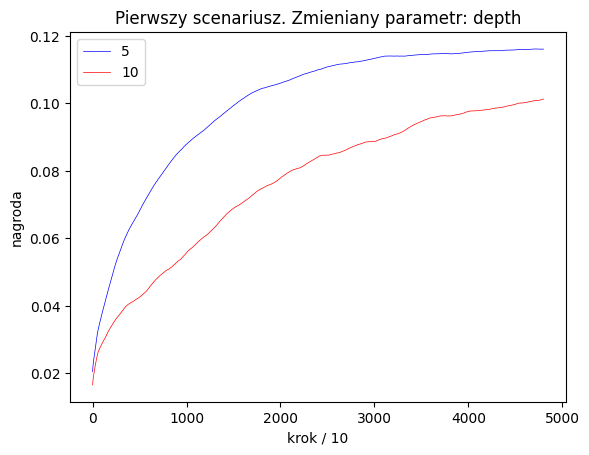
\includegraphics[width=0.5 \textwidth]{trainings/stoppingdepth}}}
    \subfloat{{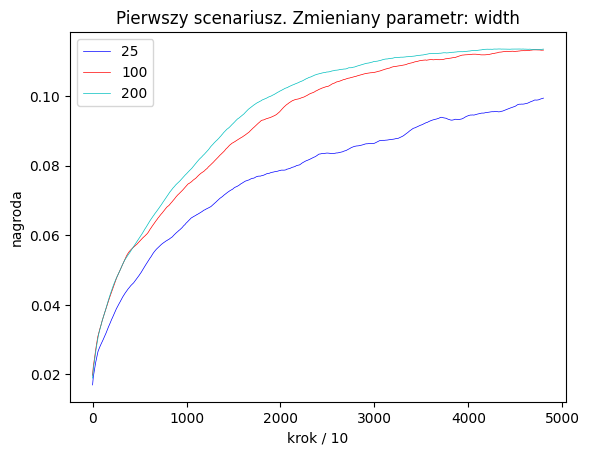
\includegraphics[width=0.5 \textwidth]{trainings/stoppingwidth}}}
    \qquad
    \subfloat{{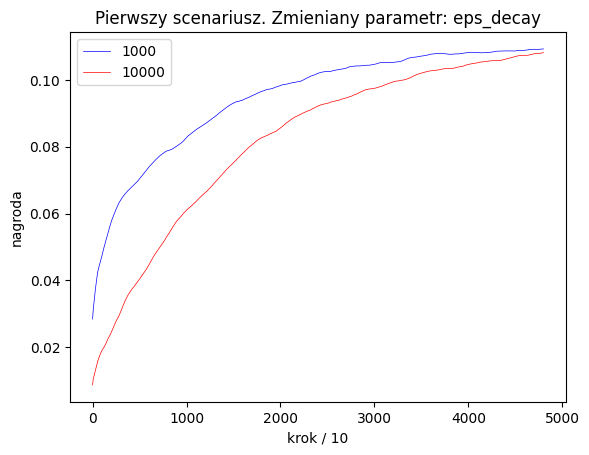
\includegraphics[width=0.5 \textwidth]{trainings/stoppingeps_decay}}}
    \subfloat{{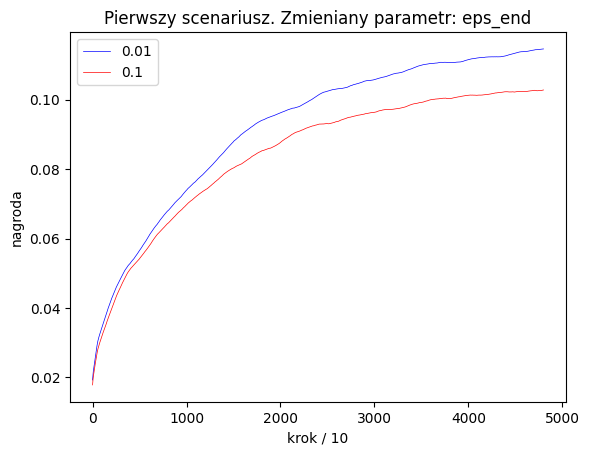
\includegraphics[width=0.5 \textwidth]{trainings/stoppingeps_end}}}
    \caption{Wpływ parametrów na zdobywaną nagrodę w~pierwszym środowisku.}
\end{figure}
Pierwszy scenariusz polegający na zatrzymywaniu pojazdu jest najłatwiejszym środowiskiem do nauczenia. Przestrzeń stanu jest najmniejsza oraz zauważalnie lepsze wyniki osiągały płytkie i szerokie sieci neuronowe.
Parametry kontrolujące sposób eksploracji wpływają na wynik treningu zgodnie z~oczekiwaniami. Większy $eps\_end$ powoduje częstsze wybieranie losowej akcji co zaniża zdobywaną nagrodę agenta dobrze dopasowanego. Mniejsza wartość $eps\_decay$ pozwala na lepsze dopasowanie agenta kosztem ilości kroków eksploracyjnych. W~dłuższym treningu lepsza eksploracja na początku uczenia mogłaby zaowocować lepszym dopasowaniem. W~trudniejszych środowiskach dłuższa eksploracja zwiększonym parametrem $eps\_decay$ może przynieść lepsze wyniki. 
\newpage
%\subsection{Trzeci scenariusz}
\begin{figure}[h]
    \subfloat{{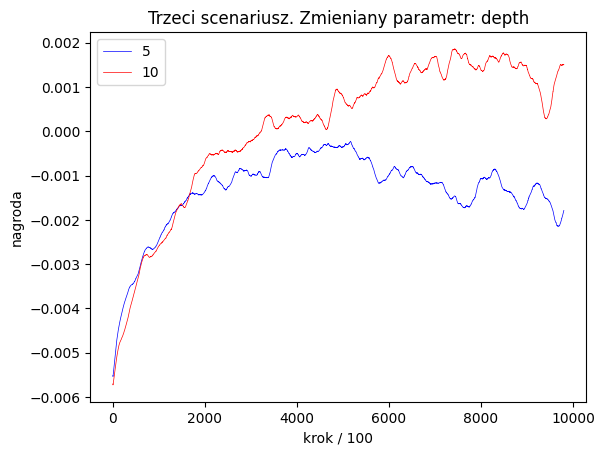
\includegraphics[width=0.5 \textwidth]{trainings/checkpoint_single_v2depth}}}
    \subfloat{{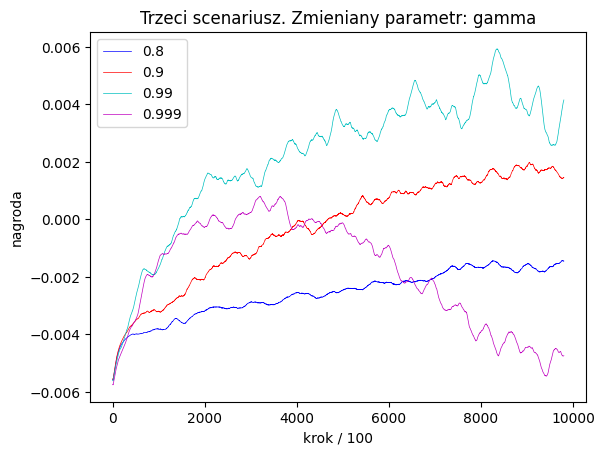
\includegraphics[width=0.5 \textwidth]{trainings/checkpoint_single_v2gamma}}}
    \qquad
    \subfloat{{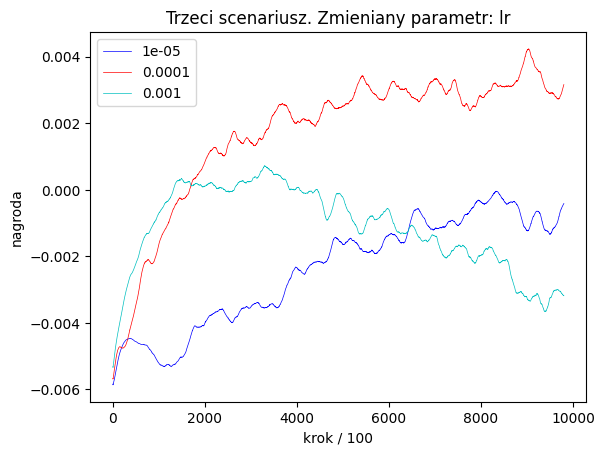
\includegraphics[width=0.5 \textwidth]{trainings/checkpoint_single_v2lr}}}
    \subfloat{{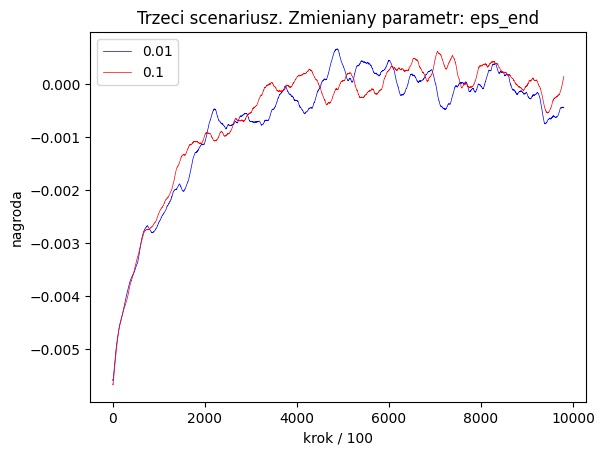
\includegraphics[width=0.5 \textwidth]{trainings/checkpoint_single_v2eps_end}}}
    \caption{Wpływ parametrów na zdobywaną nagrodę w~trzecim środowisku.}
\end{figure}
Drugi i trzeci scenariusz jest trudniejszy od pierwszego gdyż przestrzeń stanu jest większa oraz epizody są znacząco dłuższe. Zwiększenie głębokości sieci neuronowej przyniosło lepsze rezultaty. Wyraźnie widać, że parametr $gamma$ nie powinien przyjmować skrajnych wartości bliskich jeden, gdyż dochodzi do tragicznego zapominania. Mniejsza wartość tego parametru nie wpływa tak negatywnie na wydajność nauki jak za duża wartość. Krok uczący o~wielkości $lr=0.0001$ okazał się być najlepszy i~został zastosowany w~pozostałych środowiskach.
\newpage
%\subsection{Drugi scenariusz}
\begin{figure}[h]
    \subfloat{{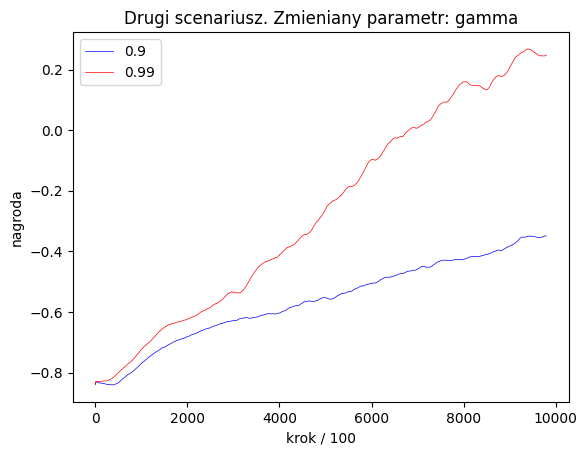
\includegraphics[width=0.5 \textwidth]{trainings/checkpoint_singlegamma}}}
    \subfloat{{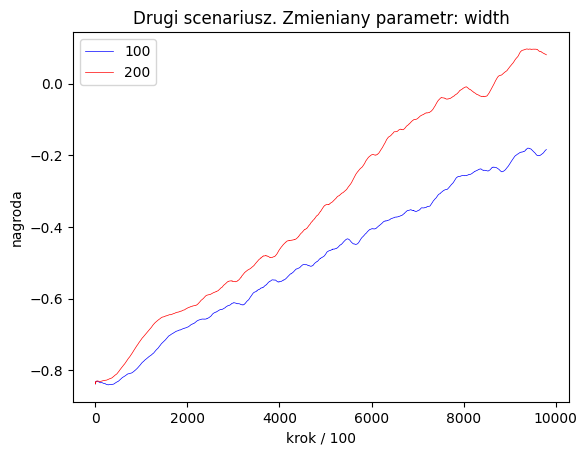
\includegraphics[width=0.5 \textwidth]{trainings//checkpoint_singlewidth}}}
    \qquad
    \subfloat{{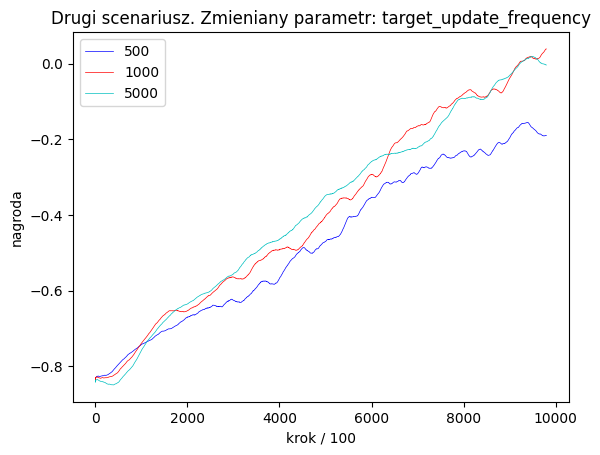
\includegraphics[width=0.5 \textwidth]{trainings/checkpoint_singletarget_update_frequency}}}
    \subfloat{{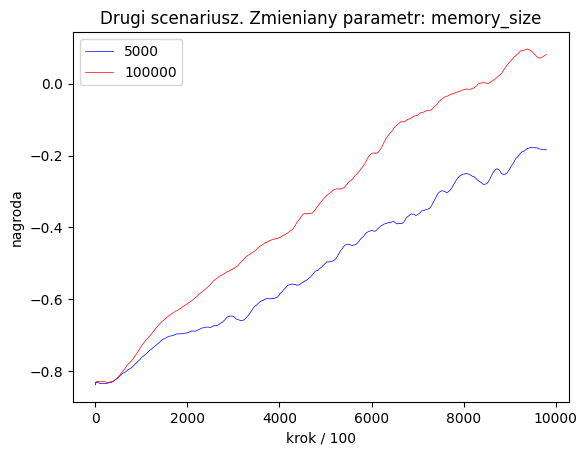
\includegraphics[width=0.5 \textwidth]{trainings/checkpoint_singlememory_size}}}
    \caption{Wpływ parametrów na zdobywaną nagrodę w~drugim środowisku.}
\end{figure}
Nietypowy, liniowy przyrost zdobywanej przez agenta nagrody wynika ze sposobu obliczania nagrody, która odpowiada zmianie odległości, a nie szybkości na którą agent ma bezpośredni wpływ. Zwiększenie pamięci poprawiło osiągane wyniki oraz stabilność treningu. Zwiększenie parametru $gamma$ kontrolującego planowanie również poprawiło wyniki. Pojawia się też zauważalny wpływ częstotliwości aktualizacji wag sieci na podstawie której obliczana jest maksymalna wartość akcji z~następnego kroku.
\newpage
Parametr living penalty, niewielka kara dawana za każdy krok, w teorii powinien zmuszać agenta do szukania bardziej ryzykownych strategii które prowadzą do szybszego zakończenia symulacji. Nagrody prezentowane na wykresach były zapisywane przed aplikacją living penalty.
\begin{figure}[h]
    \subfloat{{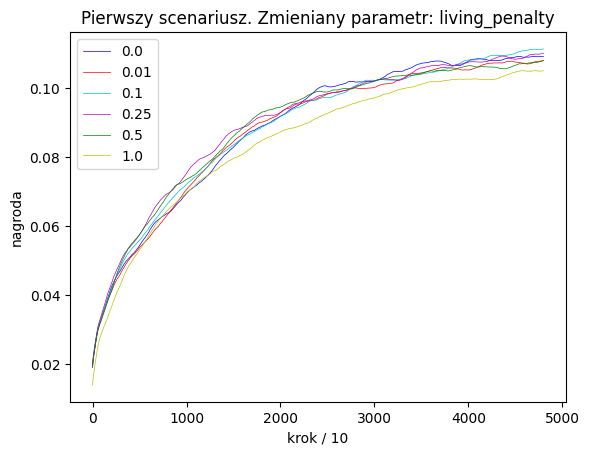
\includegraphics[width=0.5 \textwidth]{trainings/stoppingliving_penalty}}}
    \subfloat{{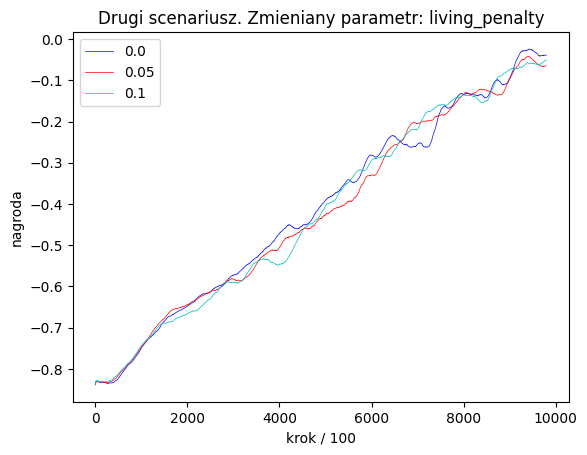
\includegraphics[width=0.5 \textwidth]{trainings/checkpoint_singleliving_penalty}}}
    \caption{Wpływ parametru living penalty na proces uczenia.}
    \label{lp}
\end{figure}
%\begin{figure}[h]
%    \subfloat{{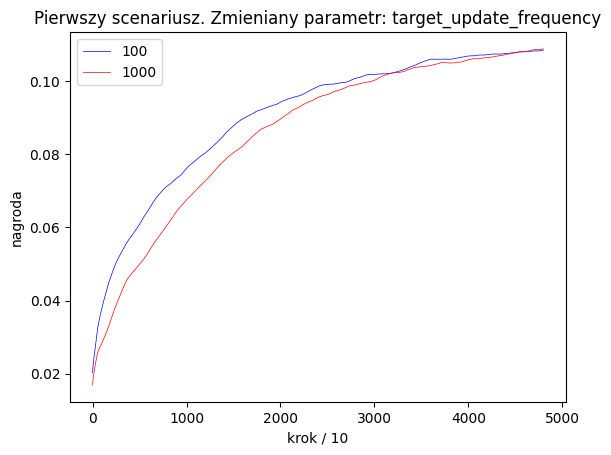
\includegraphics[width=0.5 \textwidth]{trainings/stoppingtarget_update_frequency}}}
%    \subfloat{{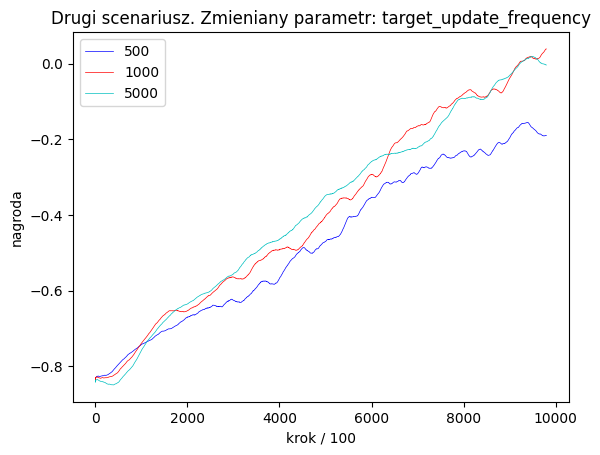
\includegraphics[width=0.5 \textwidth]{trainings/checkpoint_singletarget_update_frequency}}}
%    \caption{Wpływ parametrów na zdobywaną nagrodę w~drugim środowisku.}
%\end{figure}
\section{Wyniki testów}
Na koniec treningu zapisywane były wagi wytrenowanej sieci. Testowanie polegało na zliczaniu pojazdów, które kończyły symulację z~nagrodą (Ocalone) bądź karą (Zniszczone) w~przeciągu 10.000 kroków aktualizacji środowiska. 
Podczas testowania, podobnie jak podczas treningu, agent jednocześnie kontrolował 100 niezależnych pojazdów. Pojazd po osiągnięciu stanu terminalnego zapisywał informację o tym, czy został zniszczony czy ocalony, a następnie resetował swój stan do stanu początkowego aby kontynuować symulację. Jako że długość życia pojazdu nie jest ograniczona, agent mógł trzymać pojazd w cyklu akcji nie prowadzącym do stanu terminalnego. Na poniższych wykresach kolorem czerwonym zaznaczam najgorszego agenta, który zniszczył największą liczbę pojazdów, kolorem niebieskim najszybszego agenta, który ocalił największą ilość statków, oraz kolorem zielonym najbezpieczniejszego agenta, który miał najmniejszą ilość zniszczonych pojazdów. Otrzymaną podczas treningu nagrodę rysuję na tle nagród otrzymanych przez pozostałych agentów. Parametry odróżniające trzech agentów są zapisane w~tabelce pod wykresem. Linki znajdujące się w ostatniej kolumnie prowadzą do krótkich nagrań prezentujących zachowanie agenta. Dla zwiększenia czytelności nagrań liczba pojazdów podczas nagrywania mniejsza. Pięć pojazdów dla pierwszego scenariusza oraz 25 dla drugiego i trzeciego scenariusza. \href{https://www.youtube.com/watch?v=HJj2oh6j5uk}{Nagranie najlepszego agenta.}
%\begin{figure}[h]
%    \subfloat[Pierwszy scenariusz]{{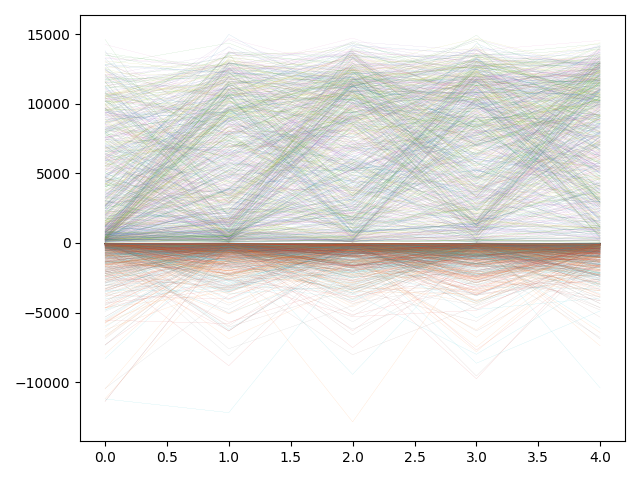
\includegraphics[wid%th=0.5 \textwidth]{stoppingtest}}}
%    \subfloat[Drugi scenariusz]{{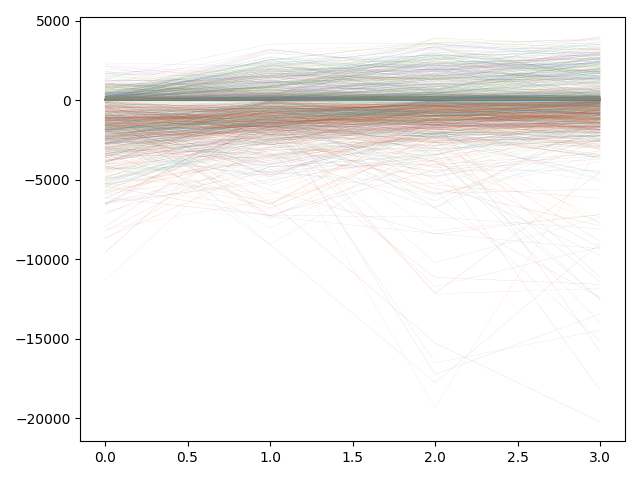
\includegraphics[width=0.5 \textwidth]{sectest}}}
%    \qquad
%    \center
%    \subfloat[Trzeci scenariusz]{{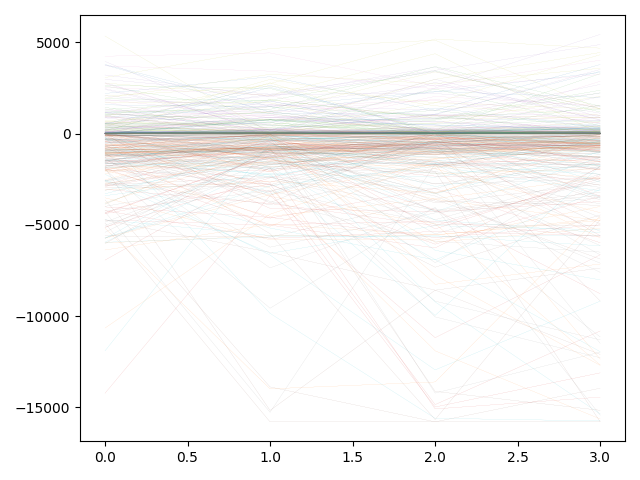
\includegraphics[width=0.5 \textwidth]{thtest}}}
%    \caption{Wyniki testów wszystkich scenariuszy.}
%\end{figure}
\newpage
%\subsection{Pierwszy scenariusz}
\begin{figure}[h]
    \subfloat{{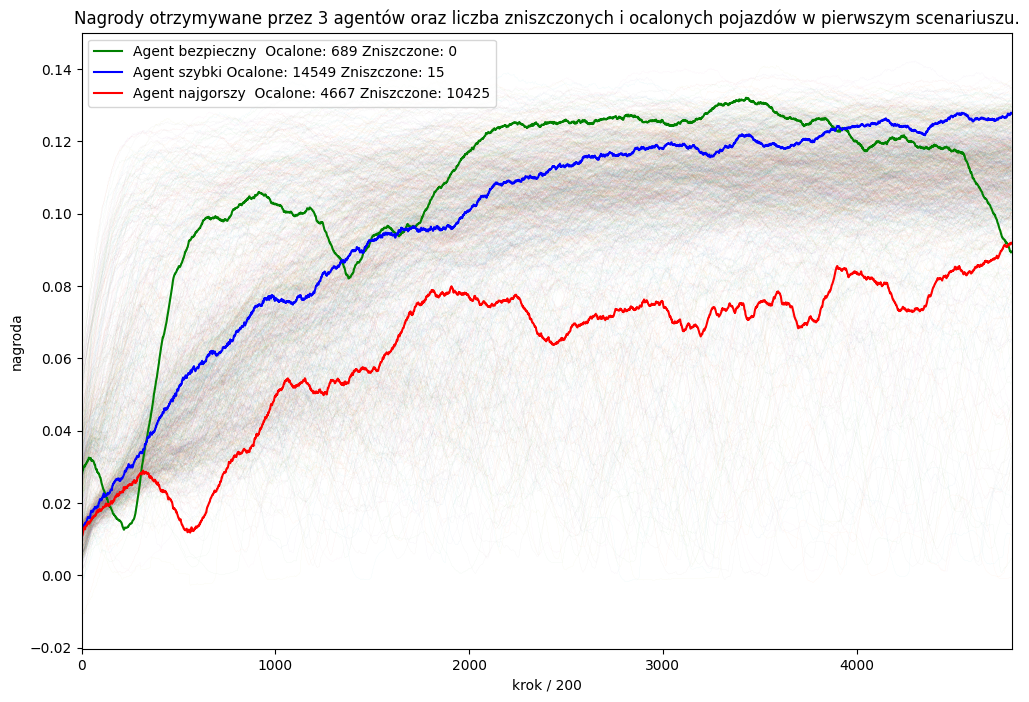
\includegraphics[width=\textwidth]{trainings/stoppingsummary}}}
    \caption{Wyniki testu w~pierwszym scenariuszu.}
\end{figure}
\begin{center}
\begin{tabular}{ |c|c|c|c|c|c|c|c|c|c|c|c|c|c|c|c|c| }
\hline
Agent & living penalty & depth & width & eps end & eps decay & batch size& video\\
\hline
Najgorszy & 1.0 & 10 & 25 & 0.1 & 10000 & 128& \href{https://youtu.be/A-l79my3kVg}{link}\\
Szybki& 0.01 & 5 & 200 & 0.01 & 10000 & 32& \href{https://youtu.be/nXtdrKZXq20}{link}\\
Bezpieczny & 0.25 & 5 & 25 & 0.01 & 1000 & 32& \href{https://youtu.be/TNg-FKpZ_yM}{link}\\
\hline
\end{tabular}
\captionof{table}{Parametry trzech wybranych agentów z pierwszego środowiska.}
\end{center}
Agent bezpieczny ocalił niecałe 700 pojazdów, podczas gdy agent szybki ocalił ich ponad 14000. Tak duża różnica wynika z tego, że pojazdu sterowane przez agenta bezpiecznego nie osiągały stanu terminalnego.
Na wykresie na Rysunku (\ref{lp}) widać, że skrajnie wysoka wartość parametru living penalty powodowała zmniejszenie otrzymywanej ze środowiska nagrody. W~pierwszym scenariuszu, gdzie maksymalna nagroda do uzyskani w pojedynczym kroku wynosi jeden, taka wartość powodowała obniżenie nagród do samych wartości ujemnych. W wyniku tego agentowi niebezpiecznemu nie zależało na odratowywaniu pojazdów które potrzebowały więcej kroków do ocalenia. Zamiast tego mniejszą karę otrzymywał przez szybkie niszczenie takich pojazdu. 
\newpage

%\subsection{Drugi scenariusz}
\begin{figure}[h]
    \subfloat{{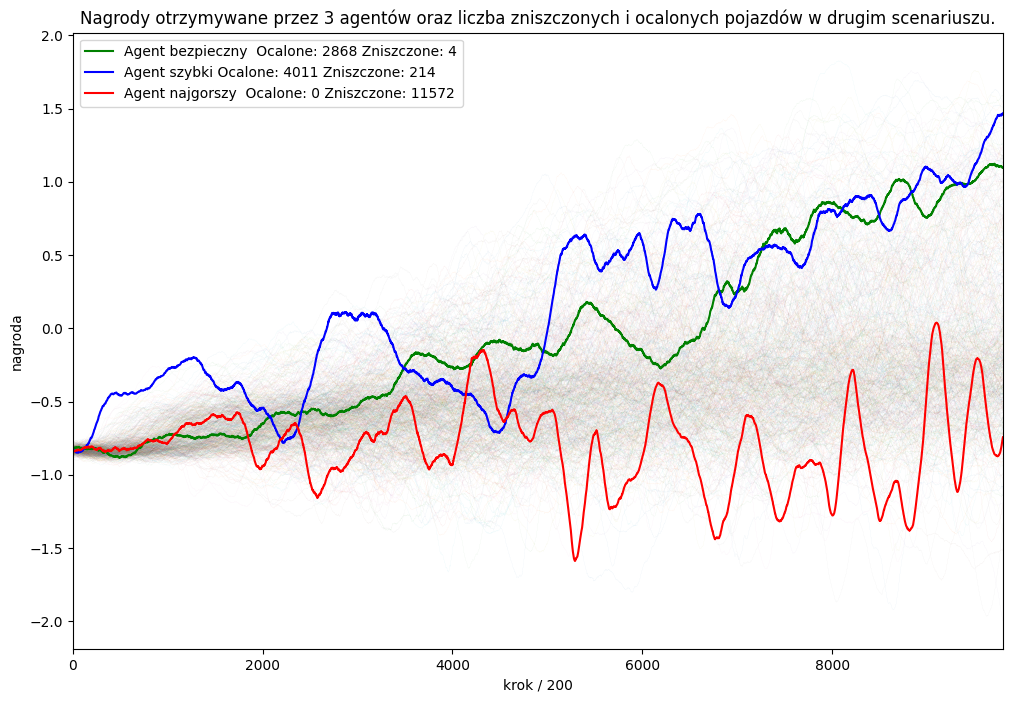
\includegraphics[width=\textwidth]{trainings/checkpoint_singlesummary}}}
    \caption{Wyniki testu w~drugim środowisku.}
\end{figure}
\begin{center}
\begin{tabular}{ |c|c|c|c|c|c|c|c|c|c|c| } 
\hline
Agent & depth & width & eps end & memory size & target update &living penalty& video\\
\hline
Najgorszy & 10 & 100 & 0.01 & 5000 & 500 &  0& \href{https://youtu.be/PT6SXxlIi_8}{link}\\
Szybki & 10 & 200 & 0.1 & 100000 & 1000 &  0.1& \href{https://youtu.be/yaug3Hmv70E}{link}\\
Bezpieczny & 20 & 200 & 0.1 & 100000 & 5000 &  0.05& \href{https://youtu.be/i--XrwREa9E}{link}\\
\hline
\end{tabular}
\captionof{table}{Parametry trzech wybranych agentów z drugiego środowiska.}
\end{center}
W~przeciwieństwie do wyników pierwszego scenariusza nic żaden parametr nie wskazuje wyraźnie na przyczynę tak złego dopasowania najgorszego agenta. Gdyby była to kwestia funkcji nagrody która uniemożliwia naukę strategii to pozostali agenci też mieliby problem z~nauką.
\newpage

%\subsection{Trzeci scenariusz}
\begin{figure}[h]
    \subfloat{{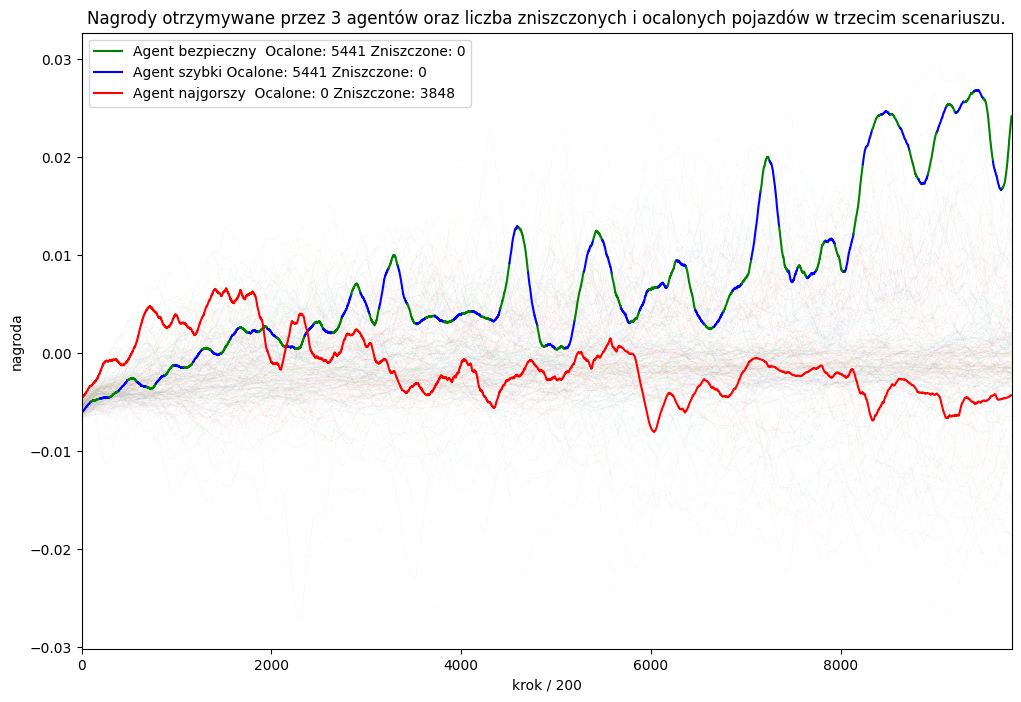
\includegraphics[width= \textwidth]{trainings/checkpoint_single_v2summary}}}
    \caption{Wyniki testu w~trzecim środowisku. Agent szybki jest jednocześnie bezpiecznym.}
\end{figure}

\begin{center}
\begin{tabular}{ |c|c|c|c|c|c|c|c|c|c|c| } 
\hline
Agent & eps end & eps decay & memory size & lr & video\\
\hline
Najgorszy & 0.1 & 100000 & 10000 & 0.001 & \href{https://youtu.be/6BRF0TOQBJI}{link}\\
Szybki i bezpieczny & 0.01 & 1000000 & 100000 & 0.0001& \href{https://youtu.be/HJj2oh6j5uk}{link}\\
\hline
\end{tabular}
\captionof{table}{Parametry trzech wybranych agentów z trzeciego środowiska.}
\end{center}
Agent który na samym początku uczenia zapowiadał się na najlepszego w~okolicy kroku 20.000 zmienił trajektorię nauki która zakończyła się najgorszym wynikiem. Porównując wyniki tego testu z~wynikami poszczególnych parametrów podczas treningu powodem tak tragicznego spadku wydajności może być za duża wartość parametru $lr$.
\newpage

%\begin{figure}[h]
%	\subfloat[Nagroda]{{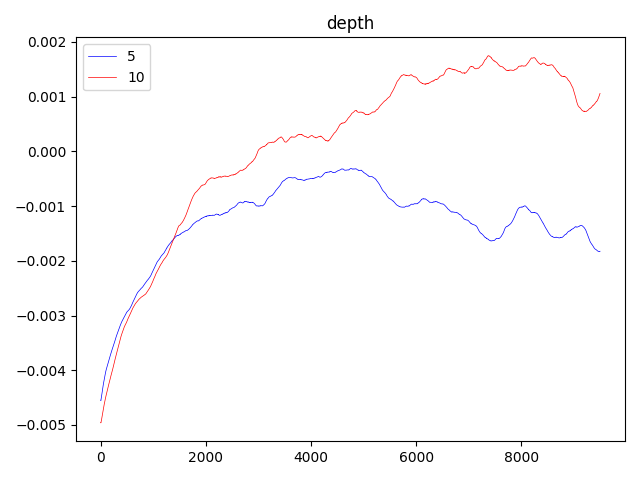
\includegraphics[width=0.5 \textwidth]{thdepth}}}
%    \subfloat[Wynik testu]{{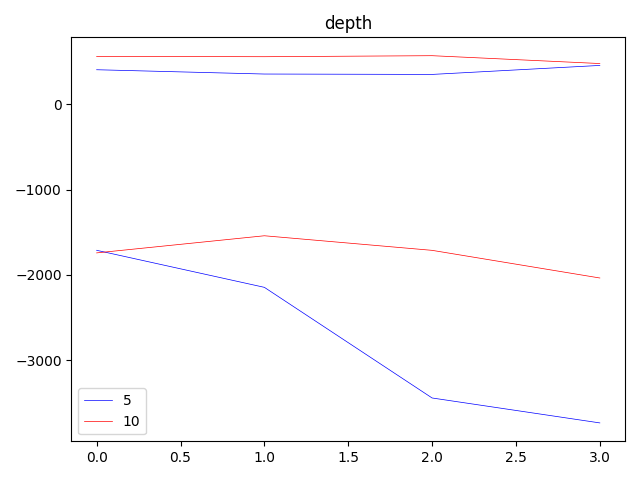
\includegraphics[width=0.5 \textwidth]{thtestdepthj}}}
%    \caption{Wyniki testu w~drugim środowisku.}
%\end{figure}

\section{Analiza trzech agentów z~pierwszego środowiska}
\begin{wrapfigure}[22]{l}{0.5 \textwidth}
\centering
\vspace{-15pt}
	\caption{Akcje wybrane podczas testów.}

	\subfloat{{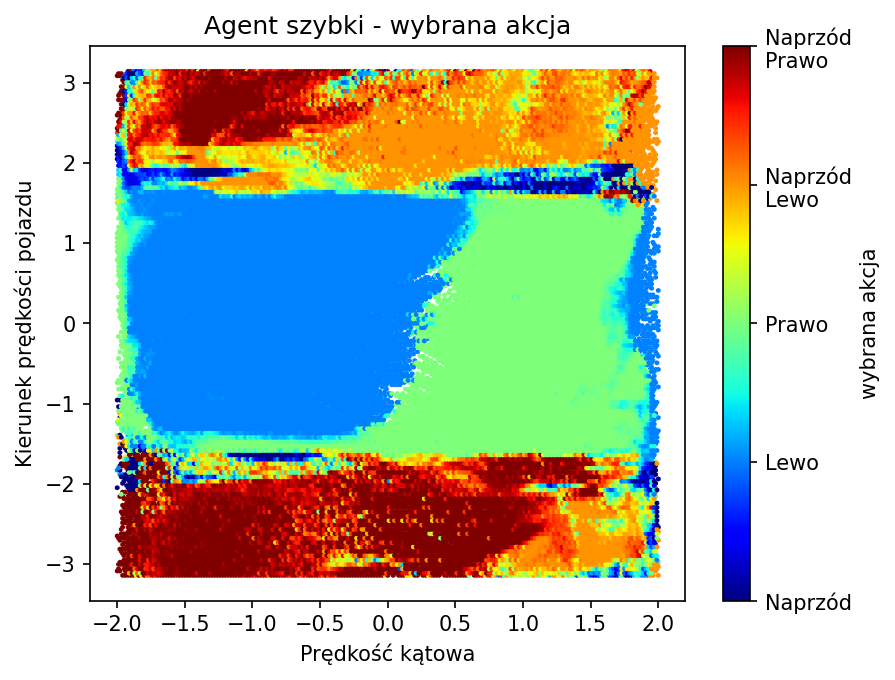
\includegraphics[width=0.5 \textwidth]{plots/FastselectedAngular_velocityShip_velocity_direction}}}
	        \qquad

	\subfloat{{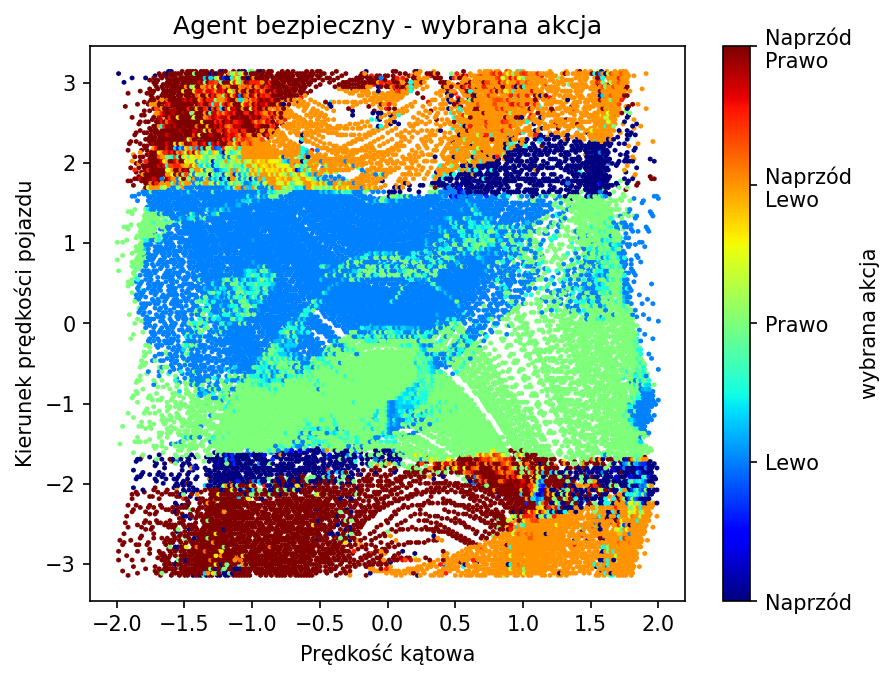
\includegraphics[width=0.5 \textwidth]{plots/SafeselectedAngular_velocityShip_velocity_direction}}}
	        \qquad

	\subfloat{{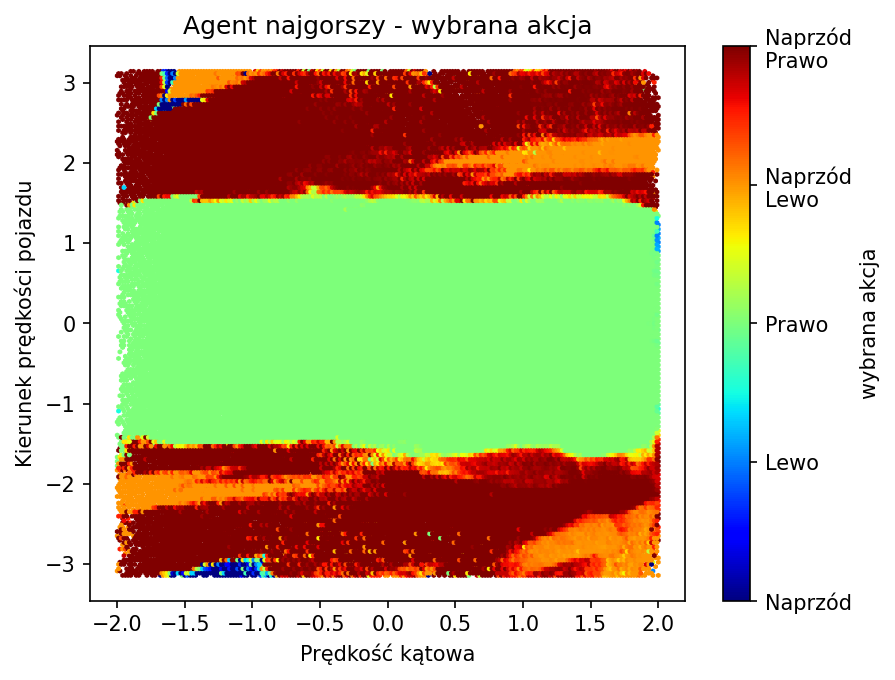
\includegraphics[width=0.5 \textwidth]{plots/DangerousselectedAngular_velocityShip_velocity_direction}}}
	\label{wybaneakcje}

\end{wrapfigure}
Na wykresach na Rysunku (\ref{wybaneakcje}) przedstawione są wybrane  podczas testowania przez agentów akcje. Stan przedstawiony jest na osiach XY, akcja wybrana w danym stanie jest zaznaczona odpowiednim kolorem. Oś X odpowiada prędkości obrotowej a~oś Y kątowi pomiędzy kierunkiem statku a~wektorem prędkości oraz prędkości kątowej. Statek zwalnia najefektywniej w~momencie kiedy pojazd zwrócony jest w~przeciwną stronę co prędkość, czyli wartość na osi Y jest bliska $\pm\pi~rad$. Agent bezpieczny ma na wykresie dużo białych plam co odpowiada braku doświadczeń z tego stanu. Wynika to z~tego, że pomimo takiej samej ilości kroków uczących i~otrzymanych obserwacji agent wybierał negującą się akcje uruchamiając na przemian prawy i~lewy silnik utrzymując stałą prędkość i~rotację pojazdu jak widać na załączonym poniżej rysunku (\ref{populacja}). Agent jest bezpieczny gdyż większość pojazdów nigdy nie kończy symulacji.
\begin{figure}[H]
\hfill\begin{minipage}{.5\textwidth}\centering
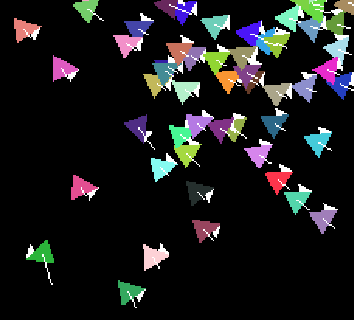
\includegraphics[width=0.7 \textwidth]{statki}
\caption{Duża część symulowanych pojazdów zablokowana w~zapętlonych akcjach przez strategię bezpiecznego agenta }
\label{populacja}
 \end{minipage}
\end{figure}
\pagebreak
Największą różnicę w wybieranych akcji (\ref{wybaneakcje}) można zaobserwować w~środkowej części wykresów, gdzie pojazd zwrócony jest przodem do kierunku lotu. Na podstawie wykresów wartości stanu na Rysunku (\ref{vval}) jest to najgorsze ułożenie pojazdu. Agent niebezpieczny prawie nie korzysta z~akcji skręcania w~lewo, co powoduje znaczną zmianę dystrybucji obserwowanych przez agenta stanów. Na wykresach prezentuję wybraną akcje w zależności od kierunku prędkości pojazdu oraz prędkości kątowej gdyż taki wykres był najbardziej czytelny. 
\begin{figure}[h]
    \caption{Dystrybucja obserwowanych stanów agenta szybkiego i niebezpiecznego. }

    \subfloat{{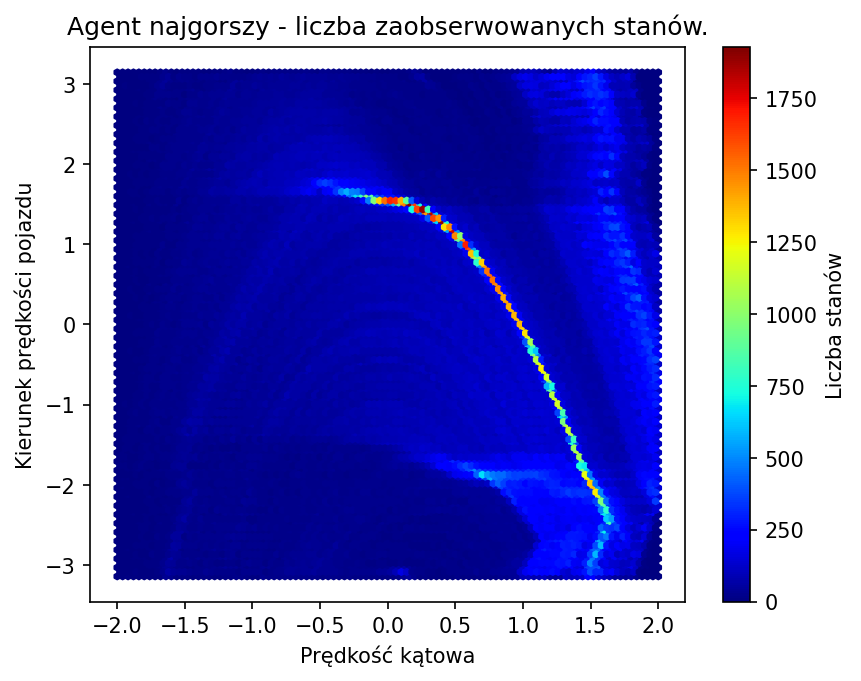
\includegraphics[height=0.3 \textheight]{plots/DangerousdistributionAngular_velocityShip_velocity_direction}}}
    \subfloat{{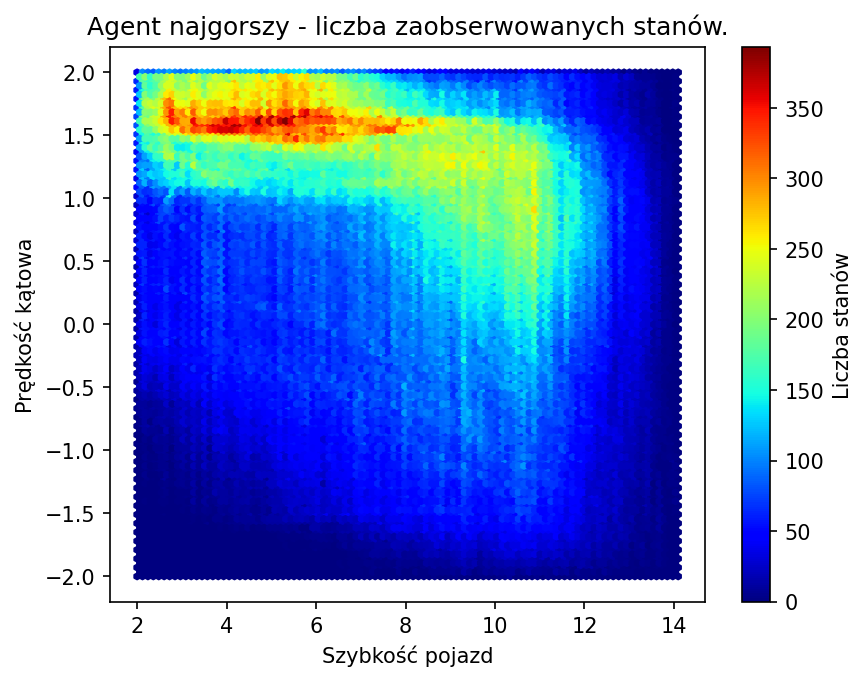
\includegraphics[height=0.3 \textheight]{plots/DangerousdistributionShip_velocityAngular_velocity}}} 
	\qquad
\subfloat{{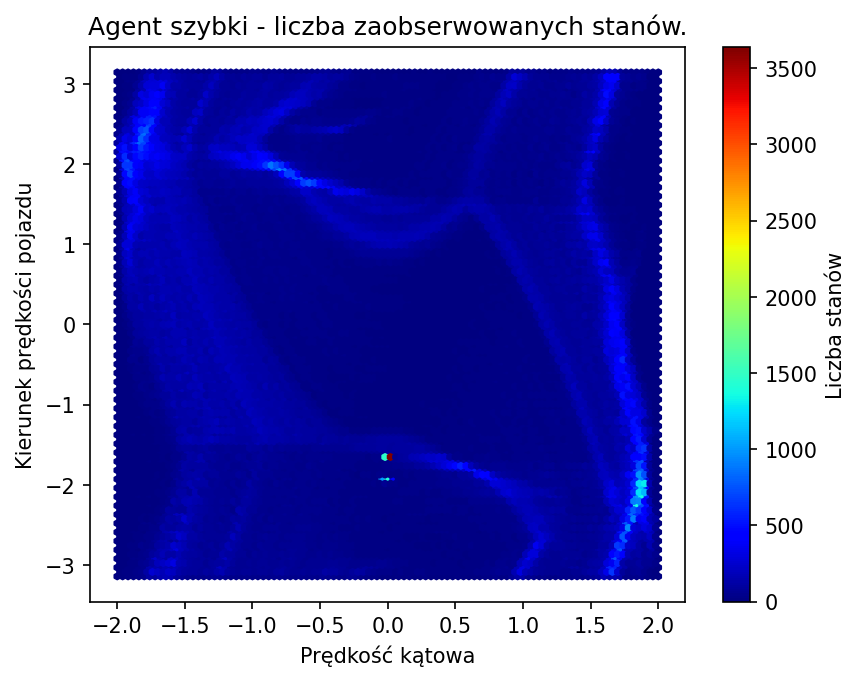
\includegraphics[height=0.3 \textheight]{plots/FastdistributionAngular_velocityShip_velocity_direction}}}
    \subfloat{{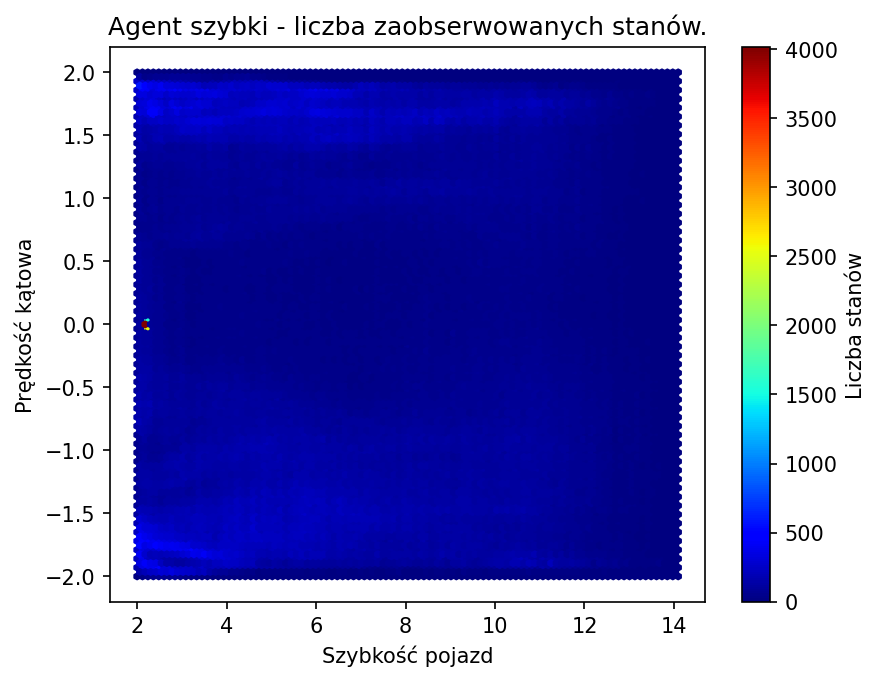
\includegraphics[height=0.3 \textheight]{plots/FastdistributionShip_velocityAngular_velocity}}} 
    \label{dystrybucja}
\end{figure}
\newpage
Różnice w nauczonych funkcjach wartości przedstawionych na wykresach na Rysunku (\ref{vval}) przez agenta szybkiego i niebezpiecznego wynikają między innymi z różnicy w parametrze living penalty wynoszącym 1 dla agenta niebezpiecznego i 0.01 dla agenta szybkiego. Wpływ preferowanej przez agenta niebezpiecznego akcji skręcania w prawo powoduje zmianę w kształcie funkcji widocznej na wykresach po prawej stronie gdzie szybkość pojazdu wynosi około $4~m/s$. Agent niebezpieczny w większości obserwowanych stanów szybko obracał się w prawą stronę, co jest widoczne na prawym górnym wykresie na Rysunku(\ref{dystrybucja}).
\begin{figure}[h]
    \caption{Wartości stanów wg agenta szybkiego i~niebezpiecznego.}

    \subfloat{{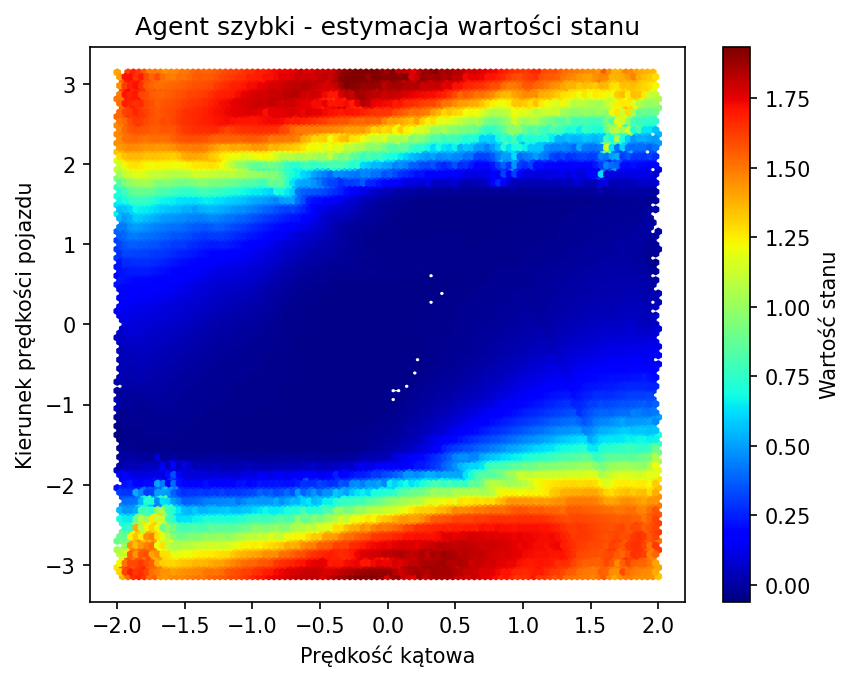
\includegraphics[height=0.3 \textheight]{plots/FaststatevAngular_velocityShip_velocity_direction}}}
    \subfloat{{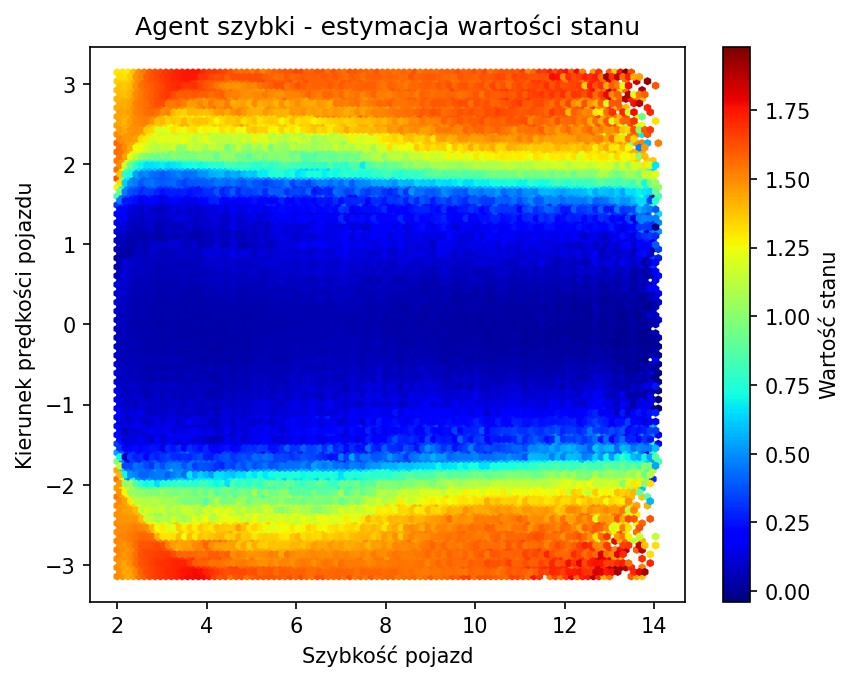
\includegraphics[height=0.3 \textheight]{plots/FaststatevShip_velocityShip_velocity_direction}}} 
        \qquad
    \subfloat{{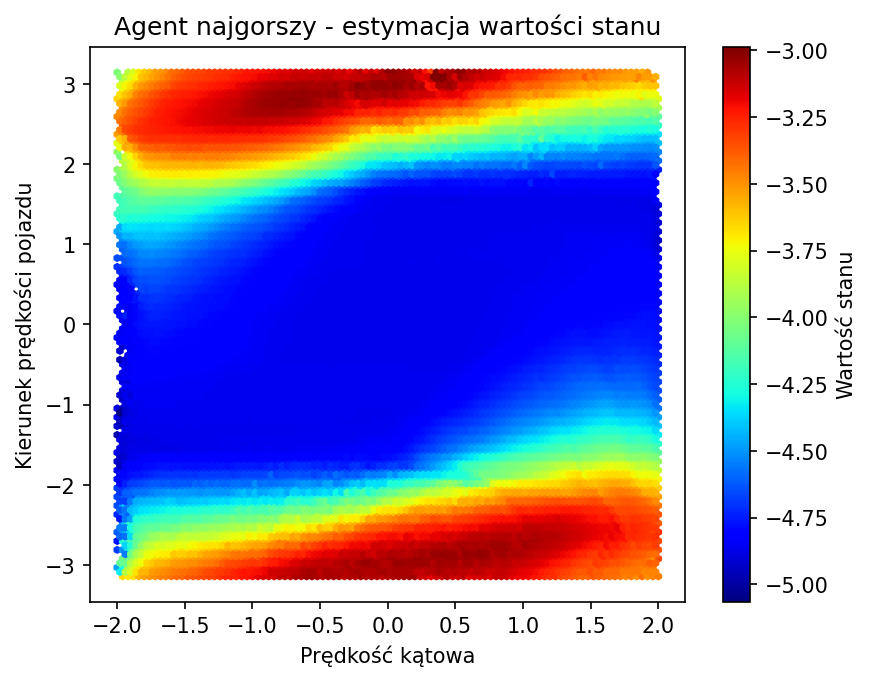
\includegraphics[height=0.3 \textheight]{plots/DangerousstatevAngular_velocityShip_velocity_direction}}}
    \subfloat{{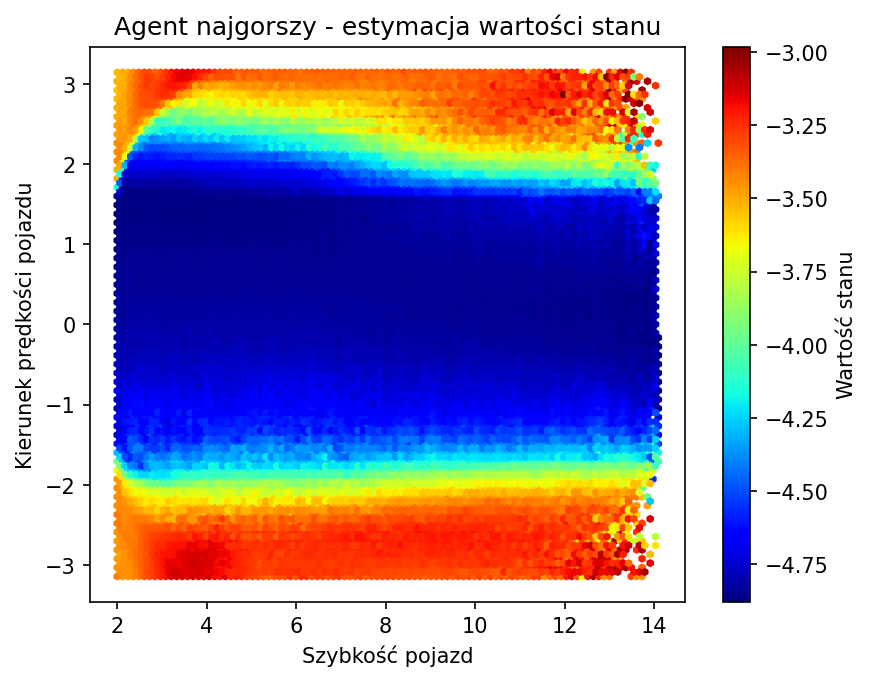
\includegraphics[height=0.3 \textheight]{plots/DangerousstatevShip_velocityShip_velocity_direction}}}   
    \label{vval}
\end{figure}
\newpage
\begin{figure}[h]
    \subfloat{{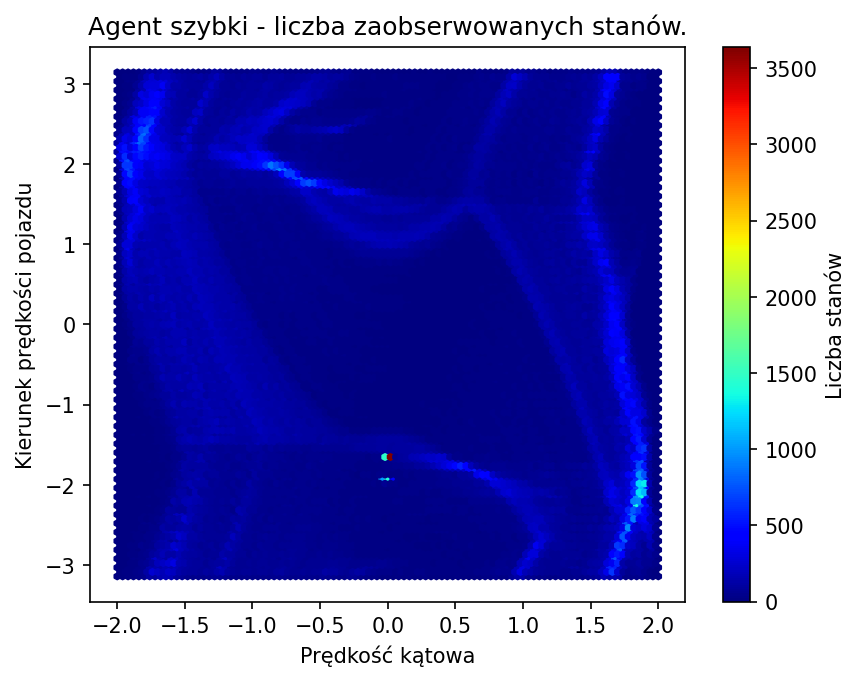
\includegraphics[height=0.3 \textheight]{plots/FastdistributionAngular_velocityShip_velocity_direction}}}
    \subfloat{{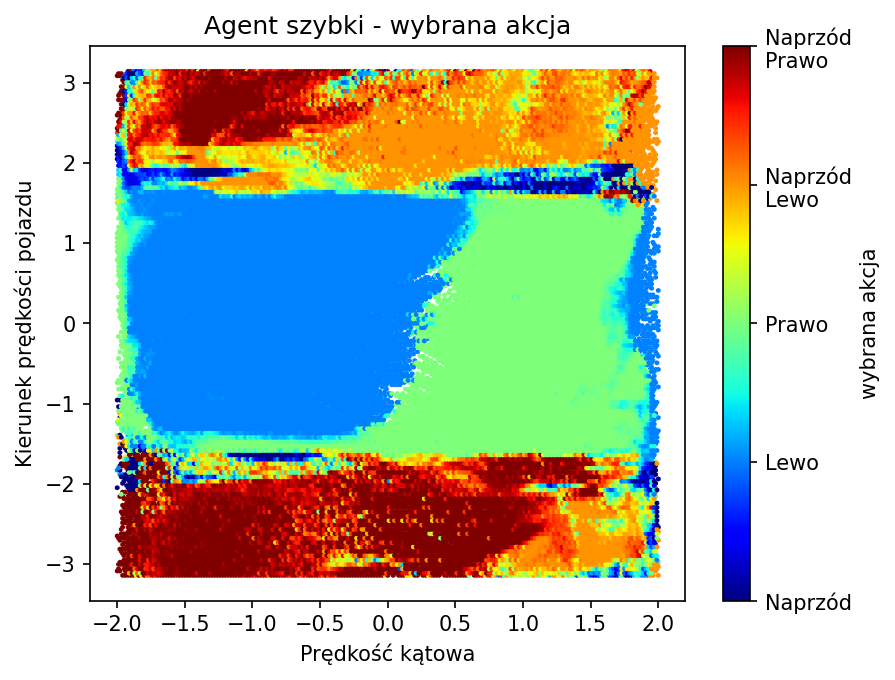
\includegraphics[height=0.3 \textheight]{plots/FastselectedAngular_velocityShip_velocity_direction}}} 
	\qquad
    \subfloat{{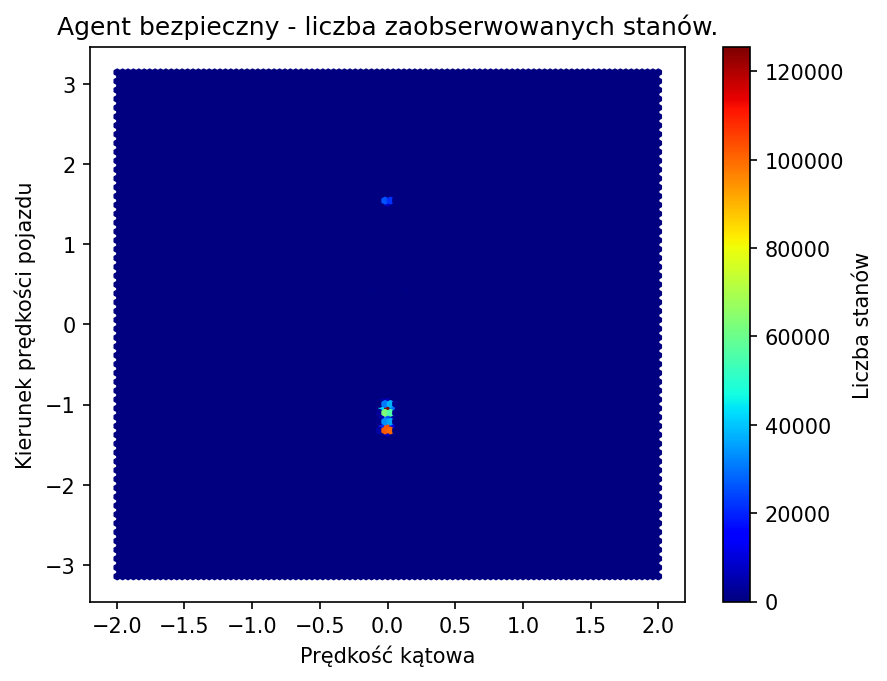
\includegraphics[height=0.3 \textheight]{plots/SafedistributionAngular_velocityShip_velocity_direction}}}
    \subfloat{{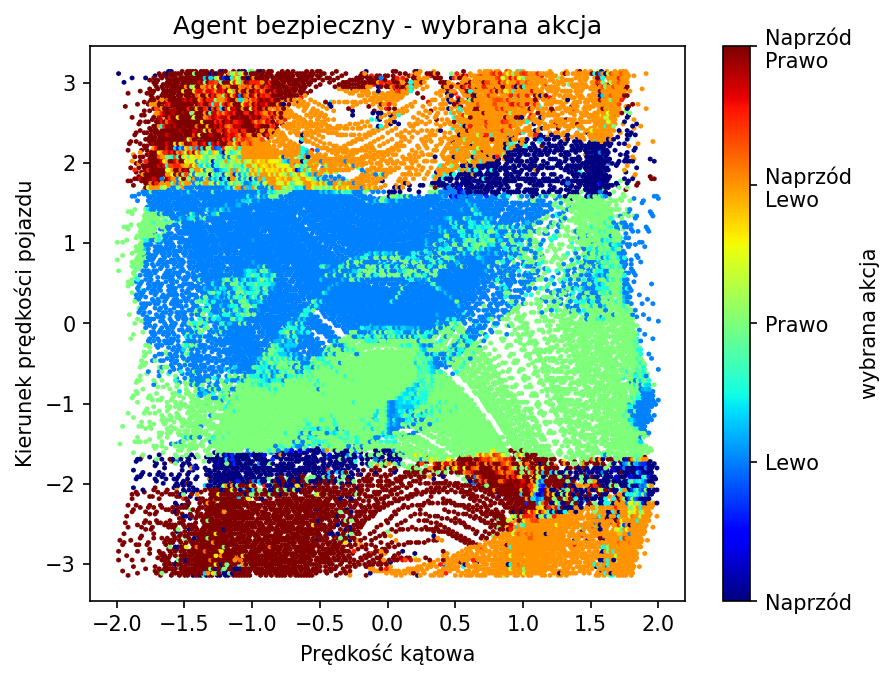
\includegraphics[height=0.3 \textheight]{plots/SafeselectedAngular_velocityShip_velocity_direction}}} 
    \caption{Obserwowane stany oraz wybrane akcje agentów bezpiecznego i szybkiego}
        \label{cykliczneakcje}

\end{figure}
Agent bezpieczny i szybki w tym samym stanie wpadają w cykl zapętlonych akcji gdzie na przemian wybierane są akcje prawo i lewo. Wskazuje na to wysoka ilość zaobserwowanych stanów w których prędkość kątowa jest bliska zeru, a kierunek prędkości pojazdu jest w zakresie $[-1,-2]$. Takie zachowanie wynika z widocznej na wykresach na Rysunku(\ref{cykliczneakcje}) po prawej stronie poszarpanej granicy pomiędzy akcją prawo i lewo.
\section{Podsumowanie}
W tej pracy udało mi się z powodzeniem nauczyć agentów sterowania pojazdami w trzech środowiskach. Wpływ poszczególnych parametrów na zdobywaną nagrodę podczas treningu i~wynik testów znacząco różni się pomiędzy scenariuszami. Wartość nagrody zdobywanej podczas treningu nie jest wystarczająca do wskazania najlepiej wytrenowanego agenta. Jeśli celem obliczeń jest wytrenowanie najlepszego agenta, odradzam korzystanie z metody przeszukiwania siatki gdyż jest niewydajna obliczeniowo. Największą korzyść podczas treningu przyniosło uczenie na podstawie wielu jednocześnie symulowanych pojazdach.

\bibliography{paper} 
\bibliographystyle{plain}
\listoffigures
\listoftables
\end{document}
